\documentclass[a4paper,AutoFakeBold,oneside,12pt]{book}
\usepackage{BUPTthesisbachelor}
\usepackage{setspace}

%\lstdefinestyle{sharpc}{language=[Sharp]C, frame=lrtb, rulecolor=\color{blue!80!black}}


%%%%%%%%%%%%%%%%%%%%%%%%% Begin Documents %%%%%%%%%%%%%%%%%%%%%%%%%%
\begin{document}

% 封面
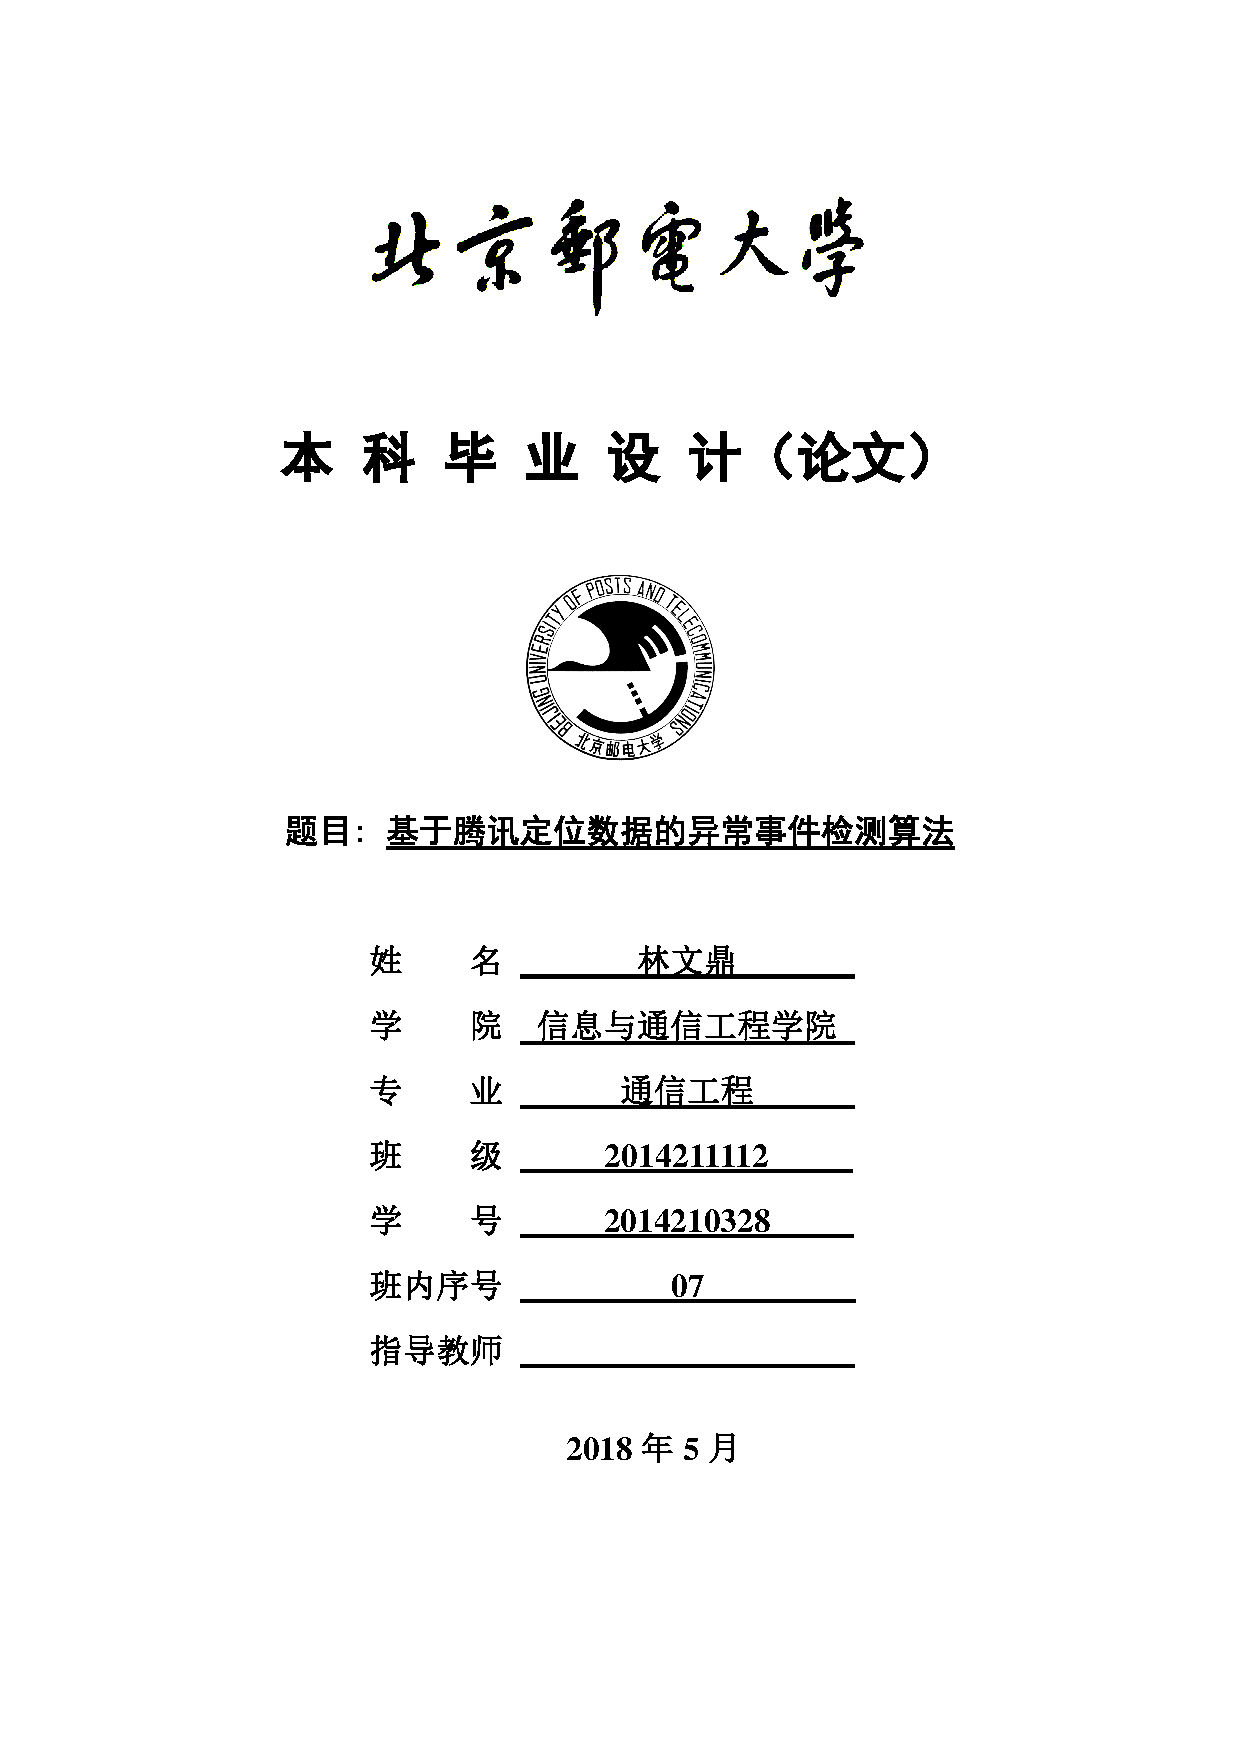
\includepdf[pages=-]{docs/cover.pdf}  
\newpage

% 任务书
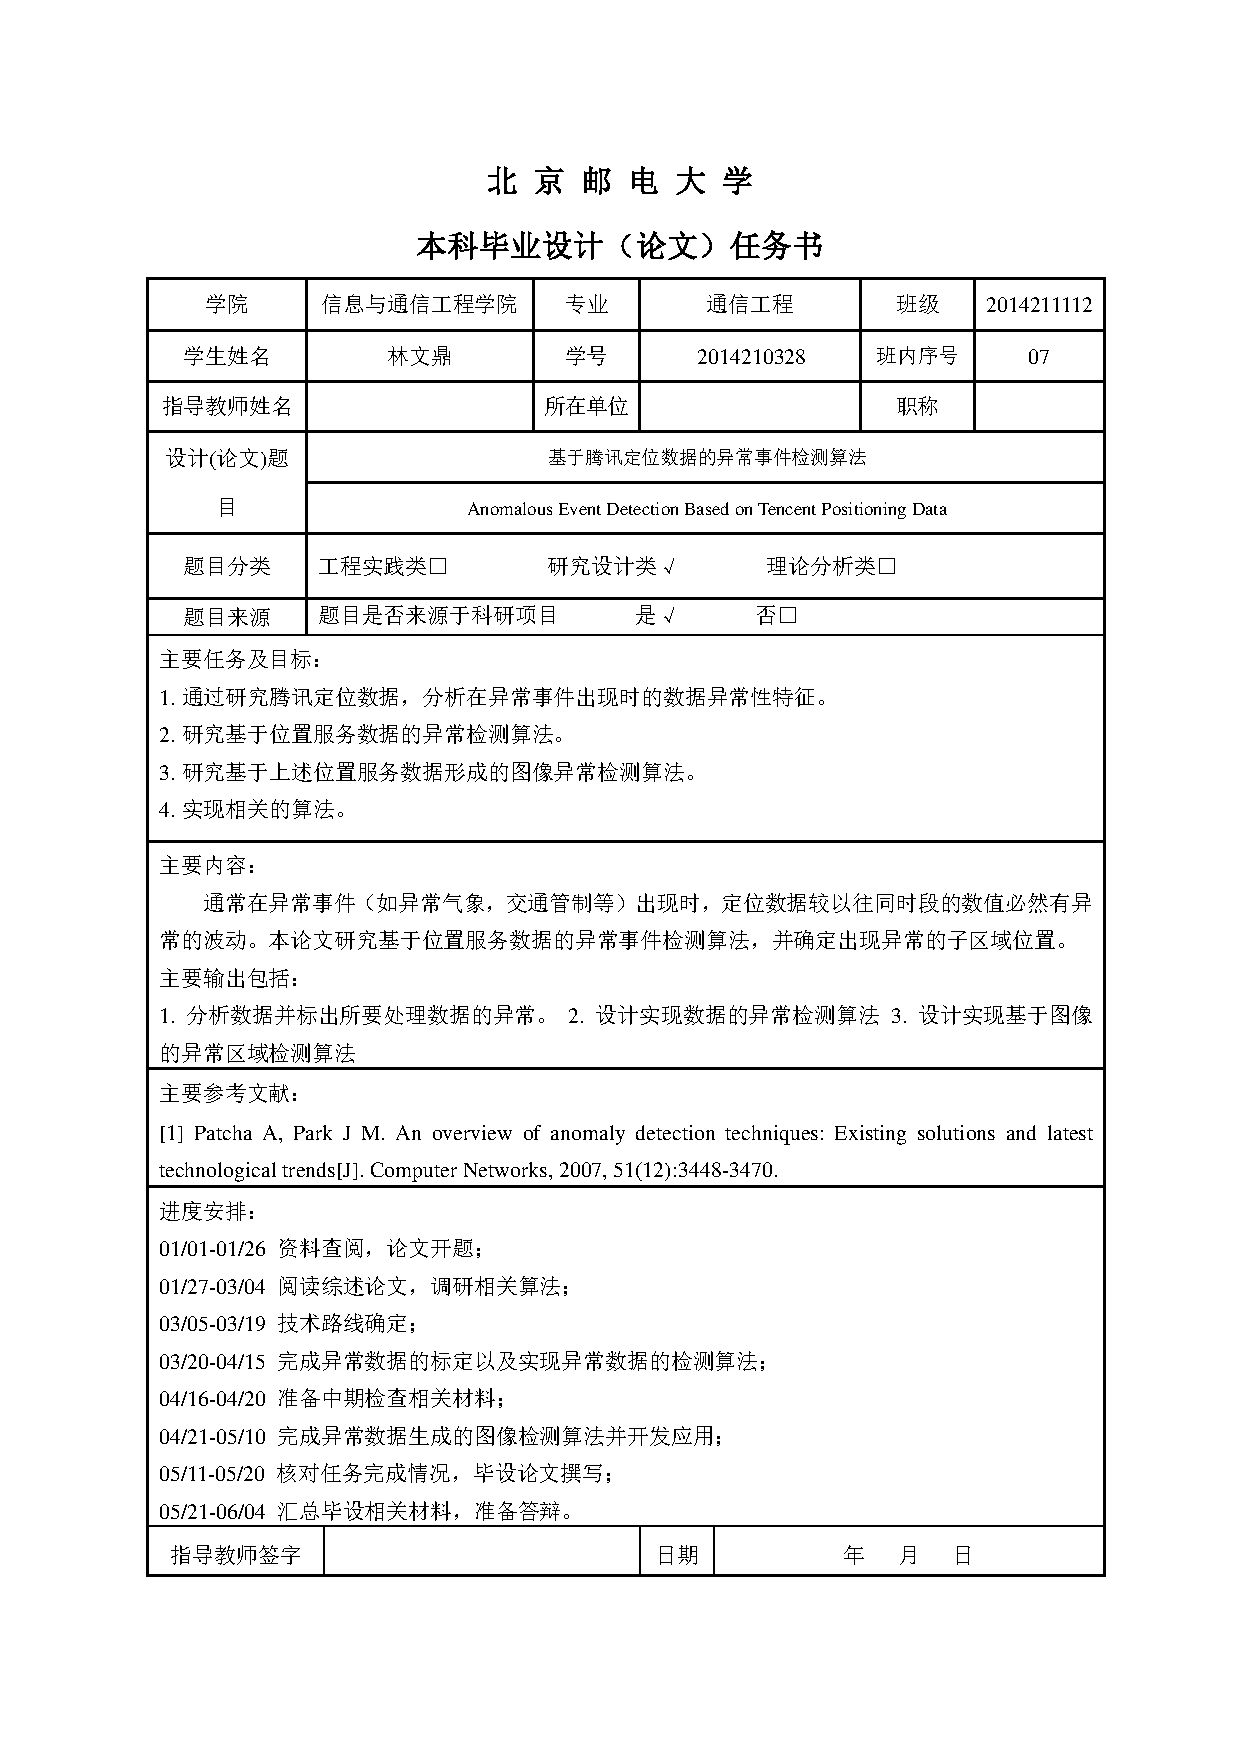
\includepdf[pages=-]{docs/task.pdf}  
\newpage

% 成绩评定表
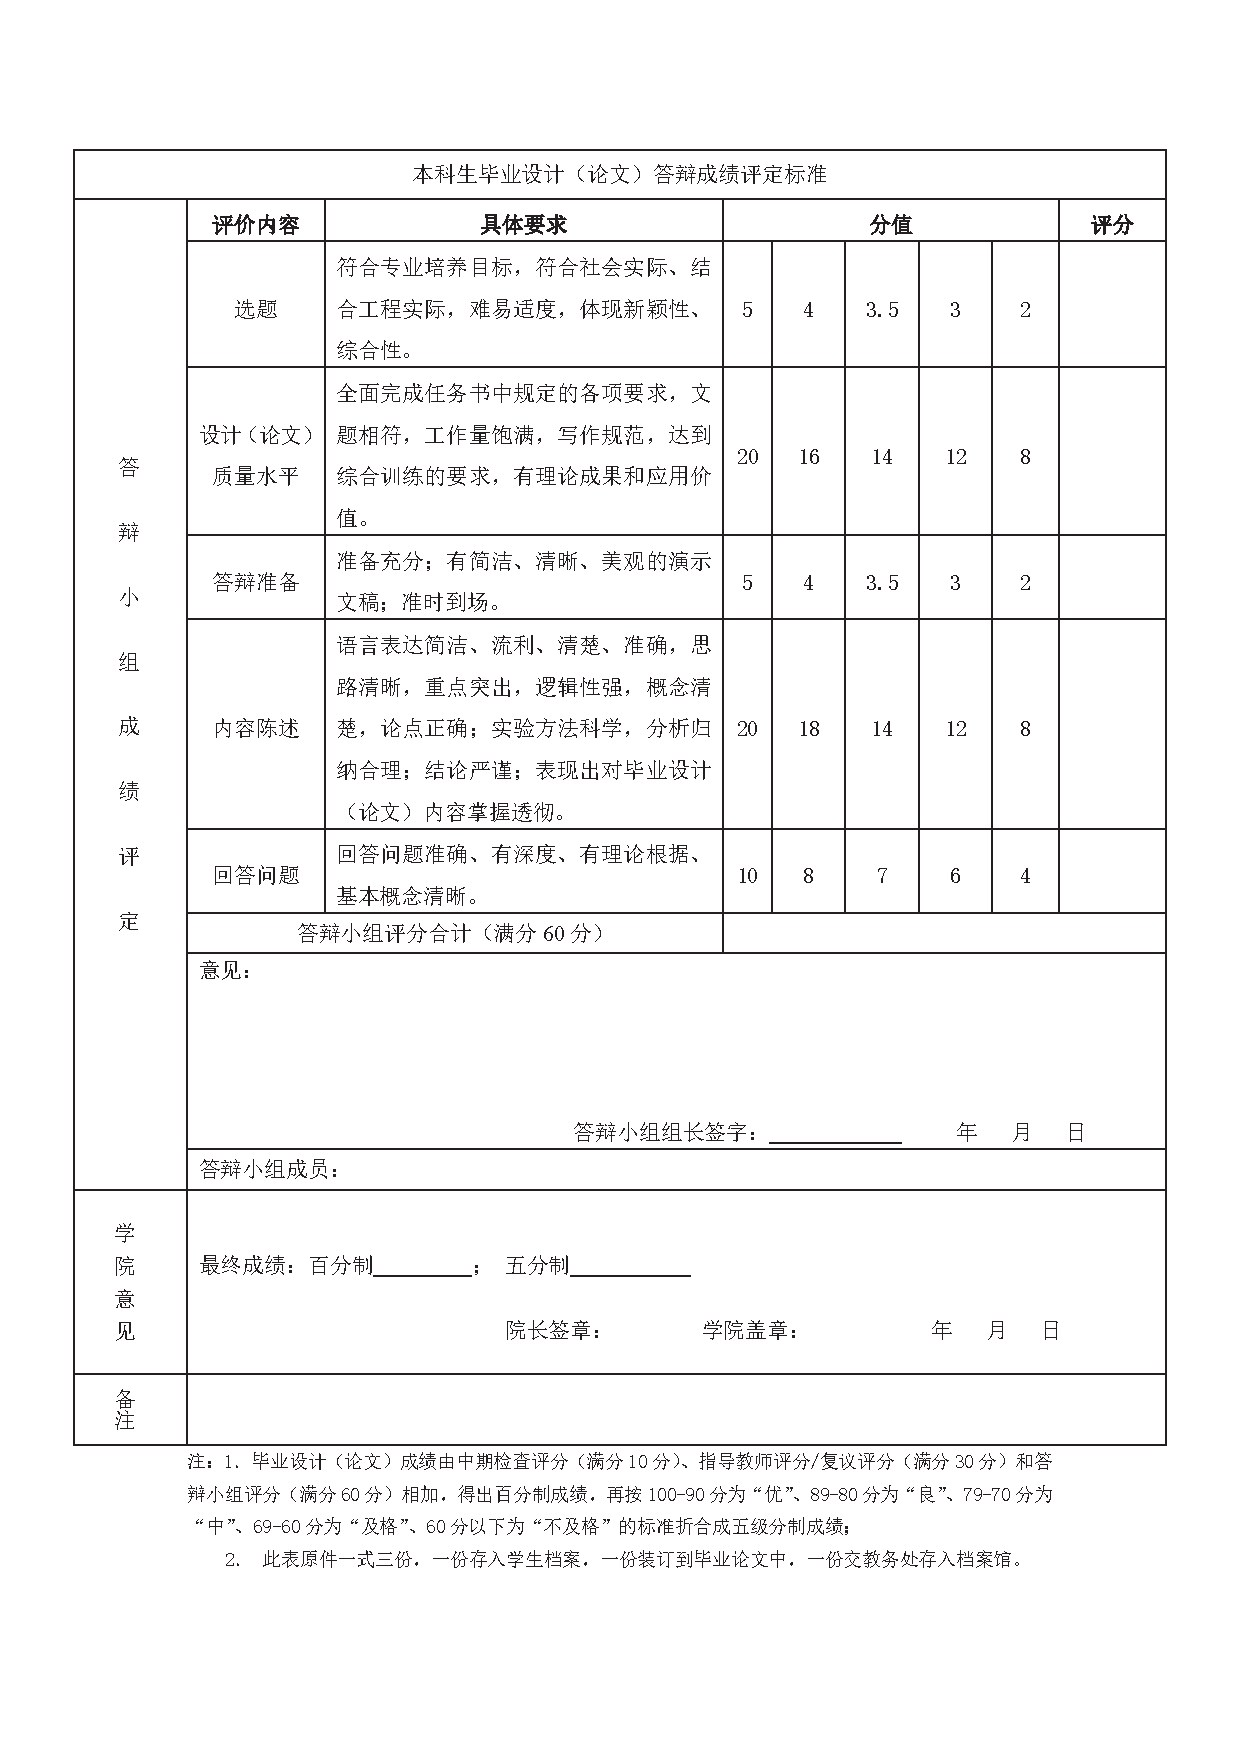
\includepdf[pages=-]{docs/scoreTable1.pdf}  
\newpage

% 诚信声明

\includepdf[pages=-]{docs/statement.pdf} 
\newpage

%%%%%%%%%%%%%%%%%%%%%%%%%%%%%%%%%%%%%%%%%%%%%%%%%%%%%%%%%%%%%%%%%%%%
%                                                                  %
%   Copyright (c) 2010 - 2011 Caspar Zhang <casparant@gmail.com>   %
%                                                                  %
%   This copyrighted material is made available to anyone wishing  %
%   to use, modify, copy, or redistribute it subject to the terms  %
%   and conditions of the GNU General Public License version 2.    %
%                                                                  %
%   This program is distributed in the hope that it will be        %
%   useful, but WITHOUT ANY WARRANTY; without even the implied     %
%   warranty of MERCHANTABILITY or FITNESS FOR A PARTICULAR        %
%   PURPOSE. See the GNU General Public License for more details.  %
%                                                                  %
%   You should have received a copy of the GNU General Public      %
%   License along with this program; if not, write to the Free     %
%   Software Foundation, Inc., 51 Franklin Street, Fifth Floor,    %
%   Boston, MA 02110-1301, USA.                                    %
%                                                                  %
%%%%%%%%%%%%%%%%%%%%%%%%%%%%%%%%%%%%%%%%%%%%%%%%%%%%%%%%%%%%%%%%%%%%

% 你只需要修改下面几行就可以完成大部分内容的填写,
% 这要求你具有一定的LaTeX基础,但是如果你足够聪明,
% 不具有LaTeX基础也可以完成。

% 论文中文题目
\def\thesistitle{基于腾讯定位数据的异常事件检测算法}

% 论文英文题目
\def\thesistitleen{Anomalous Event Detection Based on Tencent Positioning Data}

% Thank Words
\def\thankwords{

本次毕业设计是在***老师的悉心指导下完成的。从课题的选择、设计到论文的撰写一直到最后论文的定稿,期间遇到很多问题,都得到了***老师全力细心的指导。在此,向***老师表示衷心的感谢!

感谢信息与通信工程学院所有老师多年来对我的培养、帮助,使本人在本科学习中不仅学到了必备的专业知识技能和思考解决问题的方法,还学到了严谨治学的科研精神和积极进取的人生态度。

同时,感谢信息与通信工程学院的所有同学,给我创造了一个团结进取,充满温暖,充满爱的大集体,使我快乐而且充实地度过了人生中最美好的大学时光。

感谢提供此论文模板的开源项目https://github.com/sqyx008/BUPTBachelorThesis


	
}
    % Main items 
%%%%%%%%%%%%%%%%%%%%%%%%%%%%%%%%%%%%%%%%%%%%%%%%%%%%%%%%%%%%%%%%%%%%
%                                                                  %
%   Copyright (c) 2010 - 2011 Caspar Zhang <casparant@gmail.com>   %
%                                                                  %
%   This copyrighted material is made available to anyone wishing  %
%   to use, modify, copy, or redistribute it subject to the terms  %
%   and conditions of the GNU General Public License version 2.    %
%                                                                  %
%   This program is distributed in the hope that it will be        %
%   useful, but WITHOUT ANY WARRANTY; without even the implied     %
%   warranty of MERCHANTABILITY or FITNESS FOR A PARTICULAR        %
%   PURPOSE. See the GNU General Public License for more details.  %
%                                                                  %
%   You should have received a copy of the GNU General Public      %
%   License along with this program; if not, write to the Free     %
%   Software Foundation, Inc., 51 Franklin Street, Fifth Floor,    %
%   Boston, MA 02110-1301, USA.                                    %
%                                                                  %
%%%%%%%%%%%%%%%%%%%%%%%%%%%%%%%%%%%%%%%%%%%%%%%%%%%%%%%%%%%%%%%%%%%%

% 你只需要修改下面内容就可以完成中英文摘要,
% 这要求你具有一定的LaTeX基础,但是还是那句话,
% 如果你足够聪明,不具有LaTeX基础也可以完成。

% 中文摘要
\def\abstractzh{
%从这里开始写你的摘要,分段需要空一行。

通过终端设备采集的定位数据的大小反映了这个区域的人口密度特征,而通过长时记录所得到的时序定位数据更能反映密度的变化特征。人口密度的变化特征通常在时间上符合一个规律,而在某些时刻由于例如自然灾害的原因会导致该地的定位数据异常,检出这种异常能够使有关部门做好应急响应。本文基于腾讯定位数据,对确定区域的定位数据进行异常检测,研究相关的算法,并尝试确定出现异常的子区域位置。

针对以上目的,本文对给定的定位数据进行了分析及预处理,采用了基于差分、小波、极大似然估计、局部异常因子的几种曲线异常检测算法对诸如台风过境的区域全天性异常进行了检测,然后使用了非线性自回归网络基于过往时刻数据对当前时刻定位值进行曲线预测,检测了局部时刻的异常值,最后运用了帧间差分法,针对检测出的异常出现时刻使用了不同大小的滑动窗计算区域定位数据变化平均值来确定异常发生的核心子区域位置。

在基于给定的腾讯定位数据基础上,仿真结果表明:使用了曲线异常检测与预测的方法可检出区域性的整天性时段与局部性时刻异常,而通过相邻帧间差分法与滑动窗相结合能够将造成异常的主要区域检出。
%摘要结束
}

% 中文关键字 
% TODO: 改成可变长度的
\def\abszhkeyone{定位数据}
\def\abszhkeytwo{异常检测}
\def\abszhkeythree{曲线分析}

% ABSTRACT
\def\abstracten{
%Your abstract here, to make a new paragraph, give an extra blank line please.
The size of the positioning data collected by the terminal equipment reflects the population density characteristics of this area, and the time-series positioning data obtained by the long-term recording can better reflect the population density variation characteristics of the area. The characteristics of changes in population density usually conform to a rule in time. At some moments, for example, due to natural disasters, the location data of the area may be abnormal. The detection of such anomaly can enable the relevant departments to make an emergency response. In this paper, based on Tencent positioning data, we try to detect the anomaly of positioning data in a certain area, study relevant algorithms, and search the location of an abnormal sub-area in there.

For the above purposes, this paper analyzes and preprocesses the given positioning data, and adopts several curve anomaly detection algorithms based on difference, wavelet, maximum likelihood estimation, and local outlier factors for regional whole day anomaly such as typhoon crossing. Then a non-linear autoregressive network was used to curve the current local time value based on past time data to detect the hour anomaly. Finally, the inter-frame difference method was used to detect the occurrence area of the anomaly. Different sliding window sizes are used to calculate the average regional positioning data change values to determine the location of the core sub-area where the anomaly occurs.

Based on the given Tencent positioning data, the simulation results show that using the method of curve anomaly detection and prediction can detect regional all-day and local-time anomalies, and through adjacent inter-frame difference method and sliding The combination of windows can detect the main area causing the anomaly.

%Abstract done
}

% Key Words 
% TODO: 改成可变长度的
\def\absenkeyone{positioning data}
\def\absenkeytwo{anomaly detection}
\def\absenkeythree{curve analysis}



  % Abstract
\frontmatter\tableofcontents % Content

% 正文
\newpage\mainmatter
\fancypagestyle{plain}{\pagestyle{fancy}} % Add head to new chapter
\pagestyle{fancy} % Head and foot
%\let\cleardoublepagebak=\cleardoublepage
%\let\cleardoublepage\relax % Make new chapter stay on old page

%%%%%%%%%%%%%%%%%%%%%%%%%%%%% Main Area %%%%%%%%%%%%%%%%%%%%%%%%%%%%

\chapter{绪论}

% 如果你的项目来源于科研项目,可以使用以下指令插入无编号脚注于正文第一页
%\blfootnote{本项目来源于科研项目“基于\LaTeX{}的本科毕业设计”,项目编号1124}

本章主要介绍了定位数据的异常事件检测的课题背景及其研究意义,其次介绍了异常检测这一领域的基本概念及常用算法分类,最后对论文的主要研究工作进行了总结并阐述了本文的行文章节安排。

\section{课题背景}

随着GPS定位,传感器网络和高速无线通信等技术的日益发展,越来越多的终端定位数据被收集和保存在应用服务器,它们是各地人口密度的一个衡量依据。除了定位数据本身所体现的人口密度空间特征,在相同的空间位置不同的时间点上进行记录还可以得到定位数据的人口密度时序特征。而通过分析某片区域上的时序定位数据,可以得到该区域上人口密度的变化特征\cite{陈佳2014利用手机定位数据的用户特征挖掘},例如图\ref{didi}所示从北京市每日的滴滴打车的定位数据可以明显地总结出以下特征:滴滴车辆在早高峰时将大量住在郊区的人群运送至各大工作区(例如中关村和国贸区域),而在晚高峰时它们又将人群从工作区运送回家。这种区域性的时序定位数据反应出了北京市的日人口密度变化特征。



\begin{figure}[!htbp]
    \centering
    \subfloat[]{ %[]对齐方式,t为top,b为bottom,留空即可
	\label{Fig:R1} % 子图1标签名
    	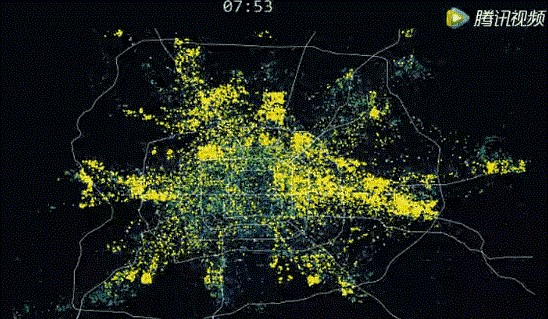
\includegraphics[width=0.45\textwidth]{pictures/1didi1} %插入图片命令,格式为[配置]{图片路径}
    }
    \quad %空格
    \subfloat[]{
	\label{Fig:R2} % 子图2标签名
    	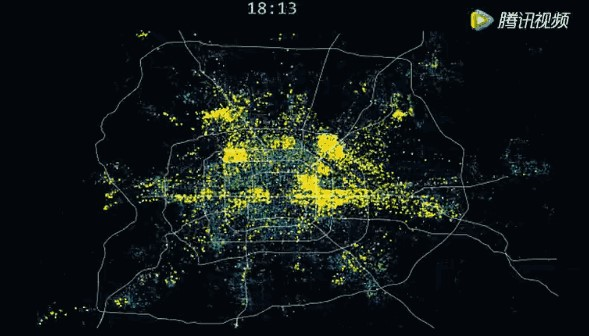
\includegraphics[width=0.45\textwidth]{pictures/1didi2}
    }
    \caption{北京市滴滴打车定位数据图} %注意须使用\protect\subref{}进行标号引用
    \label{didi} % 整个组图的标签名
\end{figure}
	而在这种区域性的时间序列中,也会在某些时间点上出现这样的观测点,它们较以往同时段的数据,例如某个月的温度与前几个月的温度变化来说,会有一个明显的波动误差,这就是时序数据点中的异常值,如图\ref{1timeano}(横坐标代表时间,纵坐标代表温度)所示,$\bm{t_1}$处和$\bm{t_2}$处的取值是一样的,但是$\bm{t_2}$属于异常点,而$\bm{t_1}$是正常的温度。分析这些异常点也是一个很重要的课题,通常对于区域性时序特征模型的建立,这些异常点是应当被剔除的噪声,它们会对模型的预测功能产生极大的阻碍。但同时异常点也可以作为一些突发事件(如异常气象,交通管制等)的判断因素,在异常事件发生时,区域的时序定位数据会在某一个时间间隔中出现较大的落差,即异常波动,通过异常检测算法将上述波动检出并分析,可以使有关部门察觉到异常状况的发生并及时做好应急响应。

\buptfigure[width=0.8\textwidth]{pictures/1timeano}{时序数据中的异常值}{1timeano}

	本课题基于腾讯定位数据,对已知的异常-某一整天确定区域的台风袭来时的定位数据进行研究,研究能够检测出该天整块区域的异常的算法,并对检测过程中的一些问题进行讨论,随后检测区域定位数据异常最大的子区域。

\section{异常检测研究现状}

\subsection{基本概念与挑战}

“异常”是指数据特征不符合该特征一般所隶属区间的现象\cite{patcha2007overview},如图\ref{1classification}所示。寻找异常是一个非常困难的课题,其难点主要来源于以下两个角度:首先,“异常”通常情况下只是一个定性的概念,偏离正常数据多少可以被界定为异常没有一个定量的比例数值,那么对于那些处于异常非异常边界线附近的异常数据来说,完全可以把边界线略微移动,使其能被归类为正常的数据;再者,用于划定数据特征正常区间的正常样本中有时也会存在异常数据,导致划定边界线偏差或是训练出的预测模型不准确。同时,考虑到正常的数据量远大于异常数据,使用机器学习的方法进行训练时很容易使网络结构偏向于正常数据的分布,即过拟合导致无法检测出异常。

\buptfigure[width=0.7\textwidth]{pictures/1classification}{点异常}{1classification}

为了便于分析,异常也有多种分类:通常情况下直观理解的异常指的是点异常,其含义是多个数据实体中,如果存在一个实体对于其他实体来说有极大的偏差,那么这个实体数据所对应的特征就表明一种点异常。而另外一种异常被称为环境异常,它与点异常中的异常概念是一样的,表征的是一个数据实体在特定环境中的异常,存在某种限定条件。这种异常类型的数据实体有两部分组成:环境属性与行为属性。环境属性表征了数据实体所处在的环境,例如时间序列数据的时间点,空间数据的地理坐标;行为属性表征了在上述特定环境属性下区分数据实体的属性,类似于地理数据的某地降雨量,行为属性即固定了环境属性后的数据特征,例如已知某地理坐标上的定位数据量。在本课题中,数据属于时序性的定位数据,而其中的异常是一种环境异常。环境属性即是时空坐标与地理坐标,行为属性是在某时间点上某地理坐标下的定位终端数量。

\subsection{异常检测算法分类}

  异常检测是找出数据特征严重不同于预期对象的一个检测过程。传统检测异常的方法分为以下几类\cite{chandola2009anomaly}:基于分类的异常检测方法,基于最近邻的异常检测方法,基于聚类的异常检测方法,基于统计的异常检测方法。

\begin{enumerate}
\item \textbf{基于分类的异常检测方法}:分类是一种从一组已做好标注的数据实例(训练)中学习模型(分类器),然后使用学习模型(测试)将测试实例分类到其中一个类中的方法。基于分类的异常检测算法以类似的两阶段方式生成一个分类模型从而判断数据的特征是否异常:在训练阶段通过使用已进行标记的样本来训练分类器的模型和参数;测试阶段使用分类器将测试实例分类为正常或异常。基于分类的异常检测算法基于以下假设下实现:在给定的数据特征空间中学习可以区分正常类和异常类的分类器是可行的。

\item \textbf{基于最近邻的异常检测方法}:近邻分析的概念已用于多种异常检测算法,这些算法都基于以下关键假设:正常的数据实例发生在密集的邻域中,而异常发生在离它们最近的邻居很远的地方。最近邻的异常检测算法需要两个数据实例之间所定义的距离或相似度衡量,而这些距离又针对不同类别的属性有不同的衡量标准。对于连续的属性,欧几里得距离的效果优秀,可以表征出两个数据间的联系性,但在不同情况下也可以使用其他方法计算。对于分类属性,通常使用简单的匹配系数,但也可以使用更复杂的距离度量。对于多变量数据实例,通常为每个属性计算距离或相似度,然后进行合并。

\item \textbf{基于聚类的异常检测方法}:聚类用于将类似的数据实例分组到集群中。尽管聚类是无监督式学习,但聚类在半监督式学习中的应用也被最近探讨。尽管聚类和异常检测看起来彼此根本不同,但是已经有几种基于聚类方法被应用于异常检测:
\begin{itemize}
\item 第一类基于聚类的算法依赖于以下假设:普通数据实例属于数据中的一个集群,而异常不属于任何集群。基于此假设的技术将已知的基于聚类的算法应用于数据集,并将任何不属于任何聚类的数据实例声明为异常。 
\item 第二类基于聚类的技术依赖于以下假设:正常的数据实例靠近它们最接近的集群质心,而异常距离它们最近的集群质心很远。基于这种假设的技术由两个步骤组成。在第一步中,数据使用聚类算法进行聚类。 在第二步中,对于每个数据实例,计算它到最近的集群质心的距离作为其异常分数。
\item 如果数据中的异常自身形成聚类,这些技术将无法检测到这种异常。为了解决这个问题,已经提出了第三类基于聚类的算法,它依赖于以下假设:普通数据实例属于大型且密集的集群,而异常集群属于小型集群或稀疏集群。基于此假设的技术将属于大小和/或密度低于阈值的集群的实例声明为异常。请注意,如果数据中的异常自身形成集群,则这些技术将无法检测到这种异常。
\end{itemize}

\item \textbf{基于统计的方法}:统计异常检测技术基于以下关键假设:正态数据实例出现在随机模型的高概率区域,而异常发生在随机模型的低概率区域。统计技术将一个统计模型(通常用于正常行为)与给定数据相匹配,然后应用统计推断测试来确定一个看不见的实例是否与该模型相符。基于应用的测试统计信息从学习模型中生成概率较低的实例被声明为异常。
\end{enumerate}

\section{论文主要工作}

本文基于以上课题背景以及研究现状,基于腾讯地图所提供的时序定位终端地图数据,在已知某一天整块定位数据区域为异常天(台风过境)的前提下,研究并实现检测出该天整块区域为异常天的算法,实现了根据现有的前几日确定时刻时序定位数据预测当前相同时刻定位数据的生成模型来处理局部时刻异常,最后使用图像处理的方法,根据异常时间点检测结果识别出造成异常的主要区域。我们对这几块内容进行了讨论,具体实现内容包含以下几部分:
\begin{enumerate}
\item \textbf{数据解析及预处理}:对腾讯定位数据进行解析及预处理。首先,由于研究的异常为台风过境时某区域的定位数异常,将定位数据的区域统一标定在该地域的经纬度;其次,对定位数据进一步作图分析,观察在相同位置处定位终端数量一天内的变化、每天同时段的变化,确定了分析已知异常的策略,讨论了处理局部时刻异常的方法;最后,根据数据特点进行预处理便于分析。
\item \textbf{基于曲线的异常检测分析}:对经过处理后的数据采取曲线分析的形式进行区域性整天异常检测。采用了诸如小波变换,极大似然估计法,差分分析法等传统方法以及一些混合改进算法,对这些算法的效果进行对比分析,根据数据结果讨论在该定位数据下对于检测整天整块区域的异常各个算法的表现。
\item \textbf{基于曲线的时序数据预测}:根据数据的分析,设计并实现曲线预测局部时刻定位数据值模型。采用动态神经网络使用现有数据中的一部分进行训练,并使用后续补充的数据进行验证,采用预测模型的方法可以有效避免只分析整天异常而无法分析小时的弊端。
\item \textbf{基于图像的异常区域检测}:在定位数据异常能够被成功检出的基础上,通过使用图像分析中的帧间差分法以及不同大小的滑动窗计算区域定位数据变化程度来确定造成整体异常的区域。
\end{enumerate}

\section{论文章节安排}

\begin{description}
\item \textbf{第一章\ 绪论}:本章主要介绍了定位数据的异常事件检测的课题背景及其研究意义,其次介绍了异常检测这一领域的基本概念及常用算法分类,最后对论文的主要研究工作进行了总结并阐述了本文的行文章节安排。
\item \textbf{第二章\ 异常检测算法基础}:本章主要介绍了异常检测的算法理论基础,涵盖后续几章所用的主要算法的一些理论背景,包括了极大似然估计,小波变换,神经网络等相关概念。
\item \textbf{第三章\ 定位数据}:本章主要介绍了本课题所研究的腾讯定位数据的形式,并在MATLAB中作图分析其数据特征,包含时序特征及地理特征,最后根据分析结果讨论如何进行检测。
\item \textbf{第四章\ 基于曲线分析的定位数据异常检测}:本章主要基于第三章数据分析的结果从曲线的角度对数据进行异常检测,研究了在数据中找出异常的方法。使用了例如小波变换、极大似然估计和邻域的方法进行了分析,并对这些方法的效果进行了讨论。
\item \textbf{第五章\ 定位数据的预测分析}:本章主要对异常检测的另一种思路进行了探讨,即实时判断数据是否异常的检测方法。采用了动态神经网络训练时序数据预测模型,并根据预测与实际值比对的结果对异常检测的效果进行了分析。
\item \textbf{第六章\ 基于区域的定位数据异常检测}:本章基于前述两章的异常检测结果,检测造成异常的重点区域。采用了图像分析的策略,例如帧间差分法,将异常的核心区域变化特征凸显并使用滑动窗标记。
\item \textbf{第七章\ 总结与展望}:本章主要对基于腾讯定位数据的异常检测算法进行分析总结,针对实验结果进行分析,获得本文方法存在的缺点并且提出解决存在问题的有效方法,提高异常检测的准确率和平台使用的有效性。
\end{description}


\chapter{异常检测算法基础}
本章主要介绍了本课题所研究的异常检测的算法基础,因为在后续几章中要根据本课题所研究的数据对象对算法进行改写,所以在本章中主要介绍理论基础,后续章节中再具体阐述实际应用策略。


\section{时序曲线离群点检测}
\subsection{极大似然估计}
	极大似然估计是一种反推样本模型参数的统计方法\cite{dempster1977maximum}。其通过对已知的样本信息建模,在数据符合某种特定分布下对分布中的参数进行似然估计。当给定了足够多的观测数据情况下,利用这些大量的试验结果去计算参数值为多少才最有可能导致这样的实验样本结果,即已经知道骰子的大量独立投掷结果去计算扔到骰子各个面的概率参数值。例如已知数据集的采样是独立且为正态分布时,我们可以使用极大似然估计法求出参数$\bm{\mu}$和$\bm{\sigma}$的值。

	设已知样本集为:$\bm{D}=\{\bm{x}_1,\bm{x}_2,\ldots,\bm{x}_N\}$

	似然函数(Link函数): 联合概率密度函数$\bm{P(D|\theta)}$称为相对于$\{\bm{x}_1,\bm{x}_2,\ldots,\bm{x}_N,\ldots\}$的$\bm{\theta}$的似然函数。

	\begin{equation}
	\bm{l(\theta)}=\bm{P(D|\theta)}=\bm{p({x}_1,{x}_2,\ldots,{x}_N|\theta)}=\bm{\prod_{i=1}^N P(x_i|\theta)}
	\end{equation}

	$\bm{\hat{\theta}}$值是未知的参数值,我们要对其进行估计,如果它的值可以在范围内使前述似然函数$\bm{l(\theta)}$的值最大,则$\bm{\hat{\theta}}$是造成这样的试验样本的最大可能值,即是$\bm{\theta}$参数的最大似然估计量。它是样本集的函数,记作:

	\begin{equation}
	\label{mlef}
	\bm{\hat{\theta}}=\bm{p({x}_1,{x}_2,\ldots,{x}_N)}=\bm{d(D)}
	\end{equation}

	在式\ref{mlef}中,$\bm{\hat{\theta}({x}_1,{x}_2,\ldots,{x}_N)}$被称作极大似然函数的估计值。

	基于上述定义,如果已知试验样本服从独立的正态分布 $\bm{N(\mu,\sigma^2)}$,则试验样本的似然函数如下式所示:

	\begin{equation}
	\bm{L(\mu,\sigma^2)}=\bm{\prod_{i=1}^N\frac{1}{\sqrt{2\pi}\sigma}e}^{-\frac{({x}_i-\mu)^2}{2\sigma^2}}=\bm{(2\pi\sigma^2)}^{-\frac{n}{2}}\bm{e}^{-\frac{1}{2\sigma^2}\sum_{i=1}^n ({x}_i-\mu)^2}
	\end{equation}

	它的对数:

	\begin{equation}
	\bm{lnL(\mu,\sigma^2)}=\bm{-\frac{n}{2}ln(2\pi)}-\bm{\frac{n}{2}ln(\sigma^2)}-\bm{\frac{1}{2\sigma^2}\sum_{i=1}^n ({x}_i-\mu)^2}
	\end{equation}

	求导,得方程组:
	
	\begin{equation}
	\begin{cases} 
	\bm{\frac{\partial lnL(\mu,\sigma^2)}{\partial \mu}}=\bm{\frac{1}{\sigma^2}\sum_{i=1}^n ({x}_i-\mu)}&=\bm{0} \\
	\bm{\frac{\partial lnL(\mu,\sigma^2)}{\partial \sigma^2}}=\bm{-\frac{n}{2\sigma^2}}+\bm{\frac{1}{2\sigma^4}\sum_{i=1}^n ({x}_i-\mu)^2}&=\bm{0}
	 \end{cases}	
	\end{equation}

	联合解得:

	\begin{equation}
	\label{mleeq}
	\begin{cases} 
	\bm{\mu^*}&=\bm{\overline{x}}=\bm{\frac{1}{n}\sum_{i=1}^n {x}_i} \\
	\bm{\sigma^{*2}}&=\bm{\frac{1}{n}\sum_{i=1}^n ({x}_i-\overline{x})^2}
	\end{cases}	
	\end{equation}

	在上述条件下,由方程式\ref{mleeq}似然方程存在唯一的解$\bm{(\mu^*,\sigma^{*2})}$:而且它一定是最大值点,这是因为当$\bm{|\mu|}\to\bm{\infty}$或$\bm{\sigma^2}\to\bm{\infty}$或$\bm{0}$时,非负函数$\bm{lnL(\mu,\sigma^2)}\to\bm{0}$。于是$\bm{\mu}$和$\bm{\sigma^{2}}$的极大似然估计为$\bm{(\mu^*,\sigma^{*2})}$。

\subsection{离散序列小波变换}

	时序信号或序列存在大量信息,但是仅仅从时序的角度去分析信号会损失大量有效信息。Fourier变换提供了一种变换域分析的方法,它利用大量的三角基去构造信号,从频域的角度对信号分析,得出更多信号的信息。

	\begin{equation}
	\bm{F(\omega)}=\bm{F[f(t)]}=\bm{\int_{-\infty}^{\infty} F(\omega)e^{-i\omega t} d\omega}
	\end{equation}

	美中不足的是,Fourier变换只能反映信号的频域特征,即将整个时序信号的频域分量提出,而不能反映各个时间点上的频域特征。短时Fourier变换(STFT)对此进行了改进,使用了定长的窗口对信号的时间进行了限制从而可以将每个短时进行Fourier频谱分析,最终得到时间轴上的频域特征。

	\begin{equation}
	\bm{X(t,\omega)}=\bm{\int_{-\infty}^{\infty} \omega(t-\tau)x(\tau)e^{-j\omega\tau} d\tau}
	\end{equation}

	小波变换是对短时Fourier变换的进一步改进\cite{portnoff1980time},与后者不同的是,小波并非使用固定的窗口去限定时间,而是使用随时间变化的窗口-小波基去构造短时的Fourier分析。它可以有效地改善STFT中对于随时间信号幅度变化很不均匀的信号无法妥善处理的缺点。

	\begin{equation}
	\bm{W_f (a,b)}=\bm{\frac{1}{\sqrt{|a|}}\int_{-\infty}^{\infty}f(t)\overline{\Psi}\frac{t-b}{a}dt}
	\end{equation}

	小波变换和Fourier变换类似,都有应用于连续信号及离散信号的分析方法。本课题所研究的时序数据应当使用离散序列小波变换,它基于Mallat算法将时序信号按照低频信号与高频信号进行逐层分解,每一层的低频信号被继续分解为低高频信号,以此类推\cite{孙延奎2009小波分析及其工程应用},具体的分解关系图\ref{2wavelet}所示:

	\buptfigure[width=0.7\textwidth]{pictures/2wavelet}{离散小波变换逐层分解图}{2wavelet}	

	时序离散序列的初始向量系数x在经过一层分解后得到高频部分$\bm{D_1}$(系数的高频部分)与低频部分$\bm{A_1}$(系数的低频部分),这两个分量是原始信号分别经过高通与低通滤波器后下采样得到的,代表着原始信号的细节以及近似部分。而后,因为$\bm{D_1}$反应的是原始信号的细节部分,继续分解没有意义,所以我们分解近似部分$\bm{A_1}$,得到二层分解的$\bm{D_2}$和$\bm{A_2}$,它们是$\bm{A_1}$信号分别经过高通与低通滤波器后下采样得到的。我们仍可以继续对$\bm{A_2}$进行分解,以此类推。由于在离散小波分解时滤波器系数G和H保持不变,所以带宽减半,但因为经过了下采样,所以每一部分仍然可以近似估计原始信号。将上述信号分解后的系数,经过正交小波基,可以还原原始信号的近似值。

\subsection{最近邻及邻域算法}

	如图\ref{2LOF1}对于$\bm{C_1}$集合里的点,它们虽然互相之间相隔较远(相对于$\bm{C_2}$来说),但它们的互相之间的间距以及分散情况是均匀的,可以认为是统一集合而不是异常的离散点。$\bm{C_2}$集合显然是统一集合,而$\bm{O_2}$虽然相对于$\bm{C_1}$集合内的点的距离是不会被认为是孤立点,但是其距离最近的$\bm{C_2}$集合相对于$\bm{C_2}$集合是较远的,即$\bm{O_2}$是异常点。LOF算法从最近邻的思想展开,提供了一种检测异常的手段。

	\buptfigure[width=0.5\textwidth]{pictures/2LOF1}{离散小波变换逐层分解图}{2LOF1}	

	首先,我们介绍LOF算法的前序概念:
	\begin{enumerate}
	\item \textbf{$\bm{d(p,o)}$}:两点$\bm{p}$和$\bm{o}$之间的距离。
	\item \textbf{k-distance(第k距离)}
	
	对于点$\bm{p}$的第k距离$\bm{d_k(p)}$定义如下:
	
	\begin{equation}
	\bm{d_k(p)}=\bm{d(p,o)}
	\end{equation}
	
	上式满足以下两个条件:
	\begin{enumerate}
	\item 在集合中至少有不包括$\bm{p}$在内的$\bm{k}$个点$\bm{o'}\in\bm{C\{x\not\equiv p\}}$,满足$\bm{d(p,o')}\leq\bm{d(p,o)}$; 
	\item 在集合中最多有不包括$\bm{p}$在内的$\bm{k-1}$个点$\bm{o'}\in\bm{C\{x\not\equiv p\}}$,满足$\bm{d(p,o')}<\bm{d(p,o)}$; 
	\end{enumerate}
	
	$\bm{p}$的第k距离,也就是距离$\bm{p}$第k远的点的距离,不包括$\bm{p}$,如图\ref{2LOF2}。 

	\buptfigure[width=0.5\textwidth]{pictures/2LOF2}{点$\bm{p}$的第5距离}{2LOF2}	

	\item \textbf{k-distance neighborhood of p(第k距离邻域)}

	点$\bm{p}$的第k距离邻域$\bm{N_k(p)}$,就是$\bm{p}$的第k距离以内的所有点,其中也包括第k距离。因此点$\bm{p}$的第k距离邻域内的点个数$\bm{N_k(p)}\ge\bm{k}$。

	\item \textbf{reach-distance(可达距离)}
	
	点$\bm{o}$到点$\bm{p}$的第k可达距离定义为:

	\begin{equation}
	\label{kreach}
	\bm{reach}-\bm{distance_k(p,o)}=\bm{max\{k-distance(o),d(p,o)\}}
	\end{equation}

	 也就是说,点$\bm{o}$到点$\bm{p}$的第k可达距离,至少是点o的第k距离,或者是$\bm{o}$和$\bm{p}$之间的真实距离。同时这也意味着,离点$\bm{o}$最近的k个点,$\bm{o}$到它们的可达距离可以认为是相等的,且都等于$\bm{d_k(o)}$
	如图\ref{2LOF3},点$\bm{o_1}$到点$\bm{p}$的第5可达距离为$\bm{d(p,o_1)}$,点$\bm{o_2}$到点$\bm{p}$的第5可达距离为$\bm{d_5(o_2)}$

	\buptfigure[width=0.8\textwidth]{pictures/2LOF3}{点$\bm{d(p,o_1)}$与点$\bm{d(p,o_2)}$到点$\bm{p}$的第5距离}{2LOF3}

	\item \textbf{ local reachability density(局部可达密度)}

	点p的局部可达密度表示为:

	\begin{equation}
	\bm{lrd_k(p)}=\bm{1}/\frac{\bm{\Sigma_{o\in N_k(p)} reach-distance_k(p,o)}}{\bm{|N_k(p)|}}
	\end{equation}

	该式的含义表示点$\bm{p}$的第k邻域内点到p的平均可达距离的倒数。 该式经常会被误解是$\bm{p}$到$\bm{|N_k(p)|}$的可达距离,其实它实际表示的是$\bm{p}$的邻域点$\bm{|N_k(p)|}$到$\bm{p}$的可达距离。并且,如果有重复点,那么分母的可达距离之和有可能为0,则会导致局部可达密度变为无限大。

	这个值的含义可以这样理解,首先这代表一个密度,密度越高,我们认为越可能属于同一簇,密度越低,越可能是离群点。如果$\bm{p}$和周围邻域点是同一簇,那么可达距离越可能为较小的$\bm{d_k(o)}$,导致可达距离之和较小,密度值较高;如果$\bm{p}$和周围邻居点较远,那么可达距离可能都会取较大值$\bm{d_k(o)}$,导致密度较小,则很可能是离群点。 
	\end{enumerate}
	
\section{时序曲线预测}
\subsection{神经网络}
	在现代信息产业中,神经网络是人们根据人脑中神经细胞中的运作原理(虽然实际上复杂的多)所模拟出来的计算系统,它通过大量的近似模拟去解决普通计算机程序无法解决的复杂问题,例如模式识别这类对人来说相对轻松的任务\cite{韩力群2005人工神经网络理论}。

	神经网络通常涉及大量处理器并行运行并按层排列的处理器。第一层接收与人类视觉处理中的视神经相似的原始输入信息,例如人眼接受的光信号在计算机中被表示为图像。每个连续的层次都接收来自其前一层的输出,而不是重新采样,越后层的神经元接受离它越近的前序神经元传来的信号。最后一层产生系统的输出。在这些一层层的神经元节点中,每一个神经元处理节点都在网络中扮演着自己的角色,即是我们无法去理解这些节点实际对信息做了什么处理,但所有的节点高度相连后,整个神经网络的输出便和输入存在某种对应关系(例如输入图像,输出判别结果)。

	神经网络在模型结构确立后,是根据训练样本来修改自身网络结构参数的,其最基本的学习集中在每一个神经元都根据前序输入进行加权,并不断权衡参数权重,使网络能够更加可能获得正确答案。通常情况下,一个网络需要经过大量已标注数据来进行训练,通过这些标注过的数据告诉网络在某种输入情况下理应输出什么,提供答案可让模型调整其内部权重,以了解如何更好地完成工作。

	最初,系数是随机的;网络创建出来时对于结构化数据一无所知。每个节点的激活函数决定了节点对一个输入或一组输入的输出。所以节点点亮与否,取决于它所接收的刺激的强度(输入和系数的返回值)是否超过了激活的阈值。在一个所谓的致密或完全连接层,每个节点的输出会传递到后续层的的所有节点。这后续会通过所有隐藏致密层,直到输出层为止,即该输入达成的决策的地方。在这个输出层,该网络关于输入的决策是针对预期决策的评估(比如,这个图片中的像素表示的是只猫还是只狗?)。通过比对网络的猜测和包含在测试集中的实际答案评估出误差,然后使用这些误差更新网络的系数,从而改变网络为图片中不同像素赋予的重要性的程度。目标是减少所形成的输出与预期输出之间的错误,正确地标识出来是狗还是猫。

	通过提供大量的网络活动日志(每行日志都有一个时间戳)给递归神经网络,递归神经网络将了解正常预期的网络活动是什么样的。当把来自于网络的陌生活动提供给训练过的网络时,它就能够区分这个活动是正常预期的,还是入侵的了。

	训练一个神经网络去识别预期行为有一个得天独厚的优势,因为它拥有大量的异常数据,或者还不足以精确分类的所有异常行为。我们在自己拥有的正常数据上训练网络,以便它能提醒我们注意未来的非正常行为。而针对攻击的训练也是在充分的数据上训练的。


\chapter{定位数据}
	本章主要介绍了本课题所研究的腾讯定位数据的基本形式,并在MATLAB中作图分析其数据特征,包含时序特征及地理特征,最后根据分析结果讨论如何进行异常检测。


\section{腾讯定位数据的形式}
	本课题所给定的腾讯定位数据是使用MATLAB的Mapping Toolbox生成的GeoTIFF格式的图像文件,每张图像文件的分辨率为113*150,文件中的Reference信息包含图像所表示的地理位置信息。本类图像数据经过处理后可以确定该图像单位像素上的值表示实际地图上的0.01经度与纬度覆盖面积上(约为平方一千米)定位终端数量,其中横坐标表示经度,纵坐标表示纬度。根据上述地理信息可以在MATLAB中画出该区域的定位终端热力图,为表现特征,采用归一化后终端定位数据作出该区域定位终端密度热力图如图\ref{3geotiff}所示:
	\buptfigure[width=0.9\textwidth]{pictures/3geotiff}{腾讯定位数据基本信息}{3geotiff}

	将地理位置信息与实际世界地图进行比对,大致确定数据坐标为广东省珠海市沿海一带,如图\ref{3matreal}所示。同时,本数据集记录了8月14日至9月30日总计48天每天的每一小时区域定位终端数量。其中,该数据中已知的异常事件为8月23日的台风过境,由于台风袭来势必会导致图上的终端定位数量发生显著改变,本课题通过分析该时段的终端定位数据来研究定位数据的异常检测方式。
	\buptfigure[width=0.9\textwidth]{pictures/3matreal}{腾讯定位数据基于的实际地理坐标上地图}{3matreal}

\section{数据分析及应用}
	对于本课题,数据的维度涵盖时间与空间,直观上要分析单日的区域性台风影响带来的异常是困难的,我们首先需要对定位数据的规律进行分析,以便确定异常检测的算法思路。
\subsection{数据的小时变化规律}

	\buptfigure[width=0.85\textwidth]{pictures/3singleday}{珠海市平均定位数据一天中随小时变化的曲线图}{3singleday}

	定位数据在时间上以小时的单位进行采样,可以通过观察某地一天24小时的终端数量值得出定位数据的小时变化规律。为便于观察,应选取终端数量较多的区域从而得出普适规律,而在3.1中我们通过比较已经确定该区域的实际地理位置,可以选择图中人口密度相对较高的珠海市进行研究。将珠海市的地理坐标范围确定后,取该区域的定位终端数量平均值并绘制出其从午夜0点至次日午夜0点的小时变化曲线图,如图\ref{3singleday}所示。

	由图\ref{3singleday}中可以看出:午夜至清晨时间段为定位终端数量最少的时间段,大多数终端处于关闭状态,这是由于在这期间用户正处于睡眠状态造成的;而随着清晨至午间及晚间的推移,用户逐渐起床、工作、娱乐,定位终端数量也能观察到数量上的上升,而后从午夜开始再次下滑。

	为确定此规律符合每一个正常的自然天,而不是工作日或休息日的特殊情况或是误采了某个节日的数据,再取该区域的定位终端数量平均值并在一张图内用不同颜色的曲线绘制出其一周每一天24小时内的小时变化曲线,如图\ref{3week}所示:

	\buptfigure[width=0.85\textwidth]{pictures/3week}{珠海市平均定位数据一周中各天随小时变化的曲线图}{3week}

	接下来我们再将一个正常天的24小时内终端数量变化的曲线与台风天的曲线进行比较,如图\ref{3normaltyp}所示:

	\buptfigure[width=0.85\textwidth]{pictures/3normaltyp}{珠海市平均定位数据在正常日与台风日随小时变化的曲线图}{3normaltyp}

	由图\ref{3normaltyp}可以分析得到数据的小时变化规律:定位终端数据在确定的地点内一周中每天的变化趋势大致相同,而对于我们所已知的台风天异常,所造成的异常影响将不仅限于某小时带来的影响,而是会对整天各个小时的数据产生大的波动。

\subsection{数据的日变化规律}
	在上一小节中,我们绘制出了台风天与正常天一天内24小时定位终端数量的变化并且观察得到台风天在一天内的值较正常值有较大的偏差。由于定位数据又在时空坐标上以自然天的单位进行采样,我们可以用同样的思路挖掘数据的日变化规律。为便于观察,同样选择图中人口密度相对较高的珠海市进行研究并选择一天当中定位终端数量较大的13:00时刻进行研究,取该区域每一天13:00的定位终端数量平均值并绘制出其在数据范围的48天内的日变化曲线图,如图\ref{3totalpart}所示:

	\buptfigure[width=0.85\textwidth]{pictures/3totalpart}{珠海市数据范围所有日期的13:00定位数据量变化曲线图}{3totalpart}

	由图\ref{3allday}中可以分析得到:在该地的每天13:00时刻,台风天相较于正常天的定位终端数有明显的偏差,是上一小节中24小时的定位终端变化曲线中的13点时刻偏差值的天数扩展。那么,如果能够通过选取任意的小时时间节点来代表整一天的定位终端数量值,台风天异常检测问题将会转化为每一天中的某确定小时的曲线异常检测问题。我们对此做进一步验证及讨论。

\subsection{数据的总时空特征}
	将上述两章所分析的小时变化规律及日变化规律进行汇总,以X轴为数据范围内的自然日,Y轴为自然日内的每一小时,在Z轴绘出XY形成的<日-时>时间节点上的定位终端数量,如图\ref{3total}所示:

\buptfigure[width=0.9\textwidth]{pictures/3total}{珠海市数据范围所有日期中定位数据量随小时变化曲线图}{3total}

	由该三维图的多角度观察可以分析得到:一天24小时内的定位数据变化确实大致相似,并且定位数据在8月23日中整体出现了一个明显的沟壑。但是,与前两小节的小部分时间节点分析不同的是,在这张图上某些小时时间点上出现了数据的突变暴露出来。如果仅依据每天中单个小时的数据对整天进行分析,过大的单小时点可能会对算法的判断产生误差;另外,由于图中仅显示了某固定点的定位数据图,需要对每个地点的时空特征进行统计,得到总体的判断依据。

\section{数据预处理及异常分析策略}

\subsection{数据预处理}
	经过3.2对数据的分析,我们得到了定位数据的基本形式同时分析了其变化规律。在3.2中,我们选取的大多是极具代表性的区域(人口密度较高的珠海市)进行分析。但实际由于该定位坐标沿海,或是从任意时间节点上的定位终端矩阵或是绘制的区域热力图中也能观察得出:位于海面上的坐标终端数值存在大量接近零的点,如图\ref{3pre}所示。这些点无论对于分析数据规律或是检测异常都是冗余的,比如海面上某点两时刻的值从1到2有100\%的变化,会极大地影响基于变化率的检测方法,需要将这些点进行剔除。

\buptfigure[width=0.85\textwidth]{pictures/3pre}{定位数据量中的高密度与低密度区域对比}{3pre}

	平均数是一个衡量区域内定位终端数量量级的基本方法,但是考虑到海面上可能会在某时刻突然出现了高额终端数这种极端异常情况,不能轻易地将其忽略。采用平均数阈值去衡量有效点可能会因为天数过多而将这种异常点舍去,因此本课题更适合采用最大值阈值的方法对数据进行预处理。

	创建一个与定位数据地图相同大小的0-1矩阵表征定位数据图中像素点是否有效(以下称为有效矩阵),读取定位数据中每一个像素点在所有时刻的值,如果这些值中没有一个超过10(1平方公里的区域中没有一个时刻超过10个定位终端),则将有效矩阵相同位置处置为0,否则置1。经过这样处理后定位数据地图中只有约2000多个点有效,极大地加快检测速度的同时也避免了突变的错误舍去。

\subsection{曲线异常分析策略}
	在第一章中我们讨论过异常的分类,而对于本课题所讨论的异常,应被归类为环境异常。环境属性即是时空坐标与地理坐标,行为属性是某地理坐标下在某时间点上的定位终端数量。台风天的检测目标即是输入所有的时空与地理坐标上的定位数据来检测出某一天的时空异常(出现台风的迹象)。

	3.2中我们讨论了数据的时空特征,对于某固定的地理坐标,其可能会在某个小时时间点上出现大的偏差,即使每天按照小时的变化定位数据的曲线大致相似,这些突然的抖动不能被忽略,所以应当使用一天中平均的定位数据来衡量。而在3.3.1中我们又对数据进行了预处理,减少了地理分析量,同时排除了一些会对算法造成影响的无效数据点。经过上述讨论,对于本课题所研究的台风天异常,对经过数据预处理后的筛选点进行时空维度上的曲线异常检测,使用每天的平均数据来分析,判断异常日期是哪一天或是全部为正常数据;再从地理上统计地图上所有已筛点的异常日期,如果地图上的大部分点都指向某一天存在异常的,即可认为该天是异常天。流程图如图\ref{3proce}所示

	\buptfigure[width=0.85\textwidth]{pictures/3proce}{基于曲线的异常检测算法步骤}{3proce}

	而对于其它类型的异常,例如某小时突然出现的剧烈抖动,由于会出现台风所造成的整体异常偏差高过该抖动的偏差的可能性,以及该剧烈抖动发生的或许只是部分区域,我们不能用上述整体区域整天的曲线分析异常检测算法来解决,对于可能的解决方案,我们将会在第5章中进行进一步讨论。


\chapter{基于曲线分析的定位数据异常检测}
	经过在第3章中对数据的分析,我们将本身<时-空>的坐标分开分析,先对单个空间上的坐标点进行时空曲线异常检测,再统计空间上的规律,得出台风异常天的检测结果。在本章中,我们对每一种方法进行了设计与验证,查看其是否能够成功检出整个区域8月23日的台风异常结果,并分析了各个算法的优势以及弊端。

\begin{algorithm} 
\floatname{algorithm}{算法}
\caption{基于曲线分析的定位数据异常检测} 
\label{a41}
\renewcommand{\algorithmicrequire}{\textbf{输入:}}
\renewcommand{\algorithmicensure}{\textbf{输出:}} 
\begin{algorithmic}[1] 
\Require 有效单个定位数据点上的日期时序定位数据值$\bm{x}=\{\bm{x}_1,\bm{x}_2,\ldots,\bm{x}_i,\ldots,\bm{x}_m\}$
\Ensure 定位数据平面上各有效点在哪天被判定为异常的日期统计图
\State 计算有效单个定位数据点上的日期时序定位数据值的平均值绘制成曲线
\State  使用曲线异常检测算法来检测出异常点$\bm{x}_a$的日期$\bm{t}_a$
\State 如果存在异常点$\bm{x}_a$,则将该日期$\bm{t}_a$的数量值$\bm{v}_a$加一
\State 以$\bm{t}$为横坐标,$\bm{v}$为纵坐标,绘制出定位数据平面上各有效点在哪天被判定为异常的日期统计图(横坐标-日期,纵坐标-该日期检测到的异常点数量)
\end{algorithmic}  
\end{algorithm}

\section{基于差分的异常检测算法}
\subsection{差分算法}
	异常是指某个数据严重偏离正常数据的范围之内,在时序数据中,如果某时刻的定位数据较其周围时刻的数据有很大的波动,该时刻的定位数据也是异常的。使用差分算法计算每一个点与其左右两个时间节点点上的数据浮动比例,当这个比例超过某种阈值后,即可认为该点是异常的。

\begin{algorithm} 
\floatname{algorithm}{算法}
\caption{基于差分的异常检测算法} 
\label{a42}
\renewcommand{\algorithmicrequire}{\textbf{输入:}}
\renewcommand{\algorithmicensure}{\textbf{输出:}} 
\begin{algorithmic}[1] 
\Require 有效单个定位数据点上的日期平均时序定位数据值$\bm{x}=\{\bm{x}_1,\bm{x}_2,\ldots,\bm{x}_i,\ldots,\bm{x}_m\}$
\Ensure 该定位数据点被判定为在$\bm{t}_a$出现异常或未出现异常
\State  计算每个数据点与周围时刻上点的差分平均值$\bm{d}_i=\frac{|\bm{x}_i-\bm{x}_{i-1}|+|\bm{x}_i-\bm{x}_{i+1}|}{\bm{x}_i}$
\State 如果存在某点$\bm{x}_a$的差分平均值$\bm{d}_a\ge20\%$,则认为该点的日期$\bm{t}_a$出现了异常;如果有多个点出现异常,选择差分平均值最大的那个点作为异常日期;如果没有异常,则无视该点继续判断其它定位数据点
\end{algorithmic}  
\end{algorithm}

\subsection{结果分析}
	采用了20\%的变化率阈值的差分算法得到了如图\ref{4laplace}所示的异常天分布情况。该图横坐标为日期,纵坐标为经过筛选后的定位点中有多少在某日期中被算法认为是异常的。由此可见本算法成功检出了异常天,并且误检率已经较低,并且由于本算法完全是线性运算,计算量较低。

\buptfigure[width=0.85\textwidth]{pictures/4laplace}{基于差分的异常检测算法定位数据异常天检出分布图}{4laplace}

	差分算法是一种更加针对平稳的时序数据算法,因为它只考虑每一个数据点相邻时序上的点,所以对于时序上突然抖动的数据更加敏感。而且,使用变化率来衡量的差分算法也对小数据的微量浮动很敏感。在本课题中,因为已经事先对数据进行预处理,排除掉了小数据的干扰才使得差分算法准确度较高。

	另外,本算法中所涉及的差分采取的是时序上左右两点间的差分值,真实异常点的附近几点也会受到异常点的影响导致可能被归类为异常点,应扩大差分的范围,减少异常点对周围点的影响。并且,实际情况中可能会出现持续的异常,此时差分方法不再适用,它只会关注陡然的变化而忽视了变化之后连续的异常,甚至还会认为持续异常之后回到正常状态的变化是异常的。

\section{基于小波变换的异常检测算法}
\subsection{离散序列小波变换}
	离散序列的小波变换基于著名的Mallat算法,离散序列值x与其第一层分解后的高频系数$\bm{D_1}$(细节部分Detail)的关系是x经过高通滤波器g滤波后再下采样,与低频系数$\bm{A_1}$(近似部分Approximate)的关系是x经过低通滤波器h滤波后再下采样;然后继续对低频系数$\bm{A_1}$进行第二层分解,依此类推,即离散信号x,经过多层分解后最后各分解系数合起来就是变换的结果。

	对于本课题的数据,因为数据规模较小,直接采用一层分解即可从原始离散序列分离出有效高频部分$\bm{D_1}$\cite{庄雪鹏2013基于小波的时间序列中异常点的检测},即原始信号的突变分量(异常分量)在$\bm{D_1}$中体现。对$\bm{D_1}$进行模糊处理并结合$\bm{A_1}$重建信号与原始信号差分\cite{张仁辉2005小波分析在信号去噪中的应用},取最大值的横坐标(日期)即可得到该地理坐标下的异常日期。

\begin{algorithm} 
\floatname{algorithm}{算法}
\caption{基于小波变换的异常检测算法} 
\label{a43}
\renewcommand{\algorithmicrequire}{\textbf{输入:}}
\renewcommand{\algorithmicensure}{\textbf{输出:}} 
\begin{algorithmic}[1] 
\Require 有效单个定位数据点上的日期平均时序定位数据值$\bm{x}=\{\bm{x}_1,\bm{x}_2,\ldots,\bm{x}_i,\ldots,\bm{x}_m\}$
\Ensure 该定位数据点被判定为在$\bm{t}_a$出现异常或未出现异常
\State  计算定位数据序列$\bm{x}$的一层离散小波变换系数$[\bm{D_1},\bm{A_1}]$
\State  对高频系数$\bm{D_1}$进行模糊处理,并结合低频系数$\bm{A_1}$重建信号$\bm{\dot{x}}$
\State 将原始信号$\bm{x}$与重建信号$\bm{\dot{x}}$进行差分,选择差分结果最大的那个点$\bm{x}_a$的日期$\bm{t}_a$作为异常日期。
\end{algorithmic}  
\end{algorithm}

\subsection{结果分析}
	使用一层的离散小波变换成功检出了异常天,如图\ref{4wave}所示,但是有数量相对较大的误检测,并且小波分解计算量较大。

\buptfigure[width=0.85\textwidth]{pictures/4wave}{基于小波变换的异常检测算法定位数据异常天检出分布图}{4wave}

	考虑到离散小波分解后是直接采用寻找最大值寻找异常天的横坐标的方法,在某些地理位置上其变化幅度较小,导致曲线本身就很平滑,采用小波变换后提取到的信号高频特征不明显,从而导致取最大值时发生错误造成了误检测。小波变换的确可以将离散的曲线信号中细微变化的部分突出,但由于台风异常的变化本身就很剧烈,导致数据的一层小波高频分量不明显。

\subsection{结果处理优化}
	在4.1.2中我们讨论的小波变换能够将时序数据的高频分量提出,进而放大原始数据的噪声异常点。但由于在这一方法中将异常放大后直接使用取最大值的策略导致很多本身没有异常的点也被错误的认为是异常点。所以,我们对该方法进行了优化,将原始时序数据经过小波分解后再进行差分运算,得到异常天出现的日期。同时,我们又对4.1中提到的差分运算运用到小波运算之中,如图\ref{4wavelet}所示。同样由于台风异常的变化本身就很剧烈,使用小波运算提取时序数据中的高频分量后再进行差分的效果不如直接对原始数据进行差分的效果好。在普通的差分算法那中,平滑的数据中出现了陡变分量则马上被检出。

\buptfigure[width=0.85\textwidth]{pictures/4wavelet}{小波变换算法处理结果优化后的定位数据异常天检出分布图}{4wavelet}

\section{基于极大似然估计的异常检测算法}
\subsection{极大似然估计与$3\sigma$准则}
	在第2章中我们讨论的极大似然估计的基本含义,其是用来估计一个概率模型的参数的一种方法,即通过若干次试验,观察其结果,利用试验结果反推最有可能(最大概率)导致这样结果的参数值。经过第3章的讨论,我们已知某地理坐标上的定位终端数在没有异常事件到来的情况下浮动规模应大致符合正态分布。基于此假设后,对于某地的时间序列求解最大似然估计,求解正态分布下似然方程得到唯一解$\bm{(\mu,\sigma^2)}$。

	在有了似然估计的解之后,我们得到了数据本身的一种拟合分布情况。在正态分布下,数值分布在$\bm{(\mu-3\sigma,\mu+3\sigma)}$中的概率为0.9973。可以认为,正态分布中Y(在本课题中为定位终端数量)的取值几乎全部集中在$\bm{(\mu-3\sigma,\mu+3\sigma)}$区间内,超出这个范围的可能性仅占不到0.3\%。本课题中所涉及的异常数据如果较正常数据偏差大,很有可能会落在此小区间中被检出,即可得到异常天的日期,否则认为不存在异常天。

\begin{algorithm} 
\floatname{algorithm}{算法}
\caption{基于极大似然估计的异常检测算法} 
\label{a44}
\renewcommand{\algorithmicrequire}{\textbf{输入:}}
\renewcommand{\algorithmicensure}{\textbf{输出:}} 
\begin{algorithmic}[1] 
\Require 有效单个定位数据点上的日期平均时序定位数据值$\bm{x}=\{\bm{x}_1,\bm{x}_2,\ldots,\bm{x}_i,\ldots,\bm{x}_m\}$
\Ensure 该定位数据点被判定为在$\bm{t}_a$出现异常或未出现异常
\State  在正态分布下求解定位数据序列$\bm{x}$的似然方程唯一解$\bm{(\mu,\sigma^2)}$
\State  寻找定位数据序列$\bm{x}$中所有处于$\bm{(\mu-3\sigma,\mu+3\sigma)}$之外的数据点
\State 如果存在这样的点$\bm{x}_a$,则认为该点的日期$\bm{t}_a$出现了异常;如果有多个点出现异常,选择差分平均值最大的那个点作为异常日期;如果没有异常,则无视该点继续判断其它定位数据点
\end{algorithmic}  
\end{algorithm}

\subsection{结果分析}
	使用极大似然估计拟合数据的分布,并基于$\bm{3\sigma}$准则将异常值筛选出后,得到了如图\ref{4like}所示的异常天分布情况。本算法仍然检出了异常天,但误检率仍然较高,且由于要求解每一个坐标点的似然估计方程,计算量相对于小波变换更加大。

\buptfigure[width=0.85\textwidth]{pictures/4like}{基于极大似然估计的异常检测算法定位数据异常天检出分布图}{4like}

	考虑到极大似然估计是基于现有的数据对原始分布进行拟合,需要较为庞大的数据量支撑以便充分拟合,才能忽略个别噪声的影。而在本课题所涉及的数据中,数据量较小且这些用来估计的现有数据中也包括了异常的数据,如果异常值偏离很大,估计出的参数会极为不准确,从而导致误检。另外,为了便于计算,本算法认为原始数据基于正态分布,实际情况下需要进行长时间的统计,对区域的定位终端数量有一个充分的采样继而判断该地的数据符合哪一种分布,最后对这种分布的参数进行极大似然估计,才能得到较为准确的模型以及判断异常的条件。

\section{局部异常因子检测算法}
\subsection{局部离群因子}

	在第2章中,我们提及了局部可达密度的概念,点p的局部可达密度表示为:

	\begin{equation}
	\label{lrdequ}
	\bm{lrd_k(p)}=\bm{1}/\frac{\bm{\Sigma_{o\in N_k(p)} reach-distance_k(p,o)}}{\bm{|N_k(p)|}}
	\end{equation}

	Breunig等人提出了局部离群因子的概念\cite{breunig2000lof},它表示点p的邻域点$\bm{N_k(p)}$的局部可达密度与点p的局部可达密度之比的平均数。 使用公式表示如下:

	\begin{equation}
	\label{lofequ}
	\bm{LOF_k(p)}=\frac{\bm{\Sigma_{o\in N_k(p)} \frac{lrd_k(o)}{lrd_k(p)}}}{\bm{|N_k(p)|}}=\frac{\bm{\Sigma_{o\in N_k(p)} lrd_k(o)}}{\bm{|N_k(p)|}}/\bm{lrd_k(p)}
	\end{equation}

	式\ref{lofequ}即局部离群因子公式的含义是点p的邻域点$\bm{N_k(p)}$的局部可达密度与点p的局部可达密度之比的平均数。

	如果比值该接近1,则p的邻域点密度相似,$\bm{p}$可能是邻域中的一个簇。如果局部离群因子的值小于1,则$\bm{p}$的密度高于邻域点密度,$\bm{p}$是稠密点。如果比值大于1,p的密度小于其邻域点密度,$\bm{p}$更可能是异常点。

	局部离群因子算法检测异常的主要思想是通过比较每个点$\bm{p}$及其邻域点的密度来确定点是否是一个异常。如果点p的密度较低,则越有可能被识别为异常。至于密度,它是由点之间的距离来计算的。点越远,密度越低,距离越近,密度越高,这完全符合我们的理解。此外,由于离群因子的值是通过点的k邻域而不是全局计算来很衡量的,所以称为“局部”异常因子,因此,对于图\ref{2LOF1}所示的两种类型数据集$\bm{C_1}$和$\bm{C_2}$,局部异常因子算法可以完全正确地处理,而不会因为数据密度分散情况不同而错误地将正常点判定为异常点。

	在本课题中的定位数据中,数据是基于时间坐标上的一维数值,但使用局部异常因子算法求解时,无需考虑数据的时刻位置,只需要关注在哪一天中数据的定位数据值与其他所有值都相差甚远,这一天即是异常出现的日子。在算法介绍的图例中考虑的距离是二维坐标上的距离,在本课题所研究的数据中,定位数据量的距离只需要用一维距离,即定位量之间的绝对值来表征。同时在使用局部异常因子算法进行求解时,可能会出现由于重复点的情况所导致的局部邻域密度值为无穷大,我们对这种情况进行特殊处理,即将重复点往周围移动1个单位,即对重复点的定位数据值+1,因为在数据分析里提及到预处理后的定位数据量至少有一天是大于5的,所以挪动1个单位对结论没有过大的影响。

\begin{algorithm} 
\floatname{algorithm}{算法}
\caption{局部异常因子检测算法} 
\label{a44}
\renewcommand{\algorithmicrequire}{\textbf{输入:}}
\renewcommand{\algorithmicensure}{\textbf{输出:}} 
\begin{algorithmic}[1] 
\Require 有效单个定位数据点上的日期平均时序定位数据值$\bm{x}=\{\bm{x}_1,\bm{x}_2,\ldots,\bm{x}_i,\ldots,\bm{x}_m\}$
\Ensure 该定位数据点被判定为在$\bm{t}_a$出现异常或未出现异常
\State  根据第2章中式\ref{kreach}计算$\bm{x}$中所有点的第k可达距离
\State  根据第2章中式\ref{lrdequ}计算$\bm{x}$中所有点的局部可达密度
\State 根据本章中式\ref{lofequ}计算$\bm{x}$中所有点的局部离群因子。如果存在这样的点$\bm{x}_a$,它的值远大于1,则认为该点的日期$\bm{t}_a$出现了异常;如果有多个点的值符合条件,选择最大的$\bm{x}_a$作为异常日期;如果没有值大于1,则无视该点继续判断其它定位数据点
\end{algorithmic}  
\end{algorithm}


\subsection{结果分析}
采用了局部离群因子来计算异常值的位置,本算法也成功检出了异常天,如图\ref{4LOF}误检率较低,但是由于局部异常因子算法需要对每个点局部异常因子进行计算,计算量复杂,效率较低。当K值(邻域范围)增加时,计算量进一步加大。

\buptfigure[width=0.85\textwidth]{pictures/4LOF}{局部异常因子检测算法定位数据异常天检出分布图}{4LOF}

局部离群因子算法与差分算法等考虑时序数据的连贯性不同,它无论时序数据还是纯粹的行为异常点都可以处理,它仅仅将数据点放置在同一张平面,用数据之间的联系来计算某点是否异常。对于K值的选择问题,由于该值的选择标准没有一个普适的定量方法,本算法采取了K=2的值\cite{杨营辉2010基于密度的样本裁剪算法的改进及在}。


\section{曲线异常检测算法总结}


\begin{bupttable}{曲线异常检测算法检测情况表}{4compa}
    \begin{tabular}{l|l|l}
		\hline \textbf{检测算法} & \textbf{异常点数}  & \textbf{运行速度(秒)} \\
		\hline 差分运算 & 909 & 1.14\\
		\hline 离散小波变换 & 191 & 7.38 \\
		\hline 小波变换-结果改进 & 293 & 8.75 \\
		\hline 最大似然法($\bm{3\sigma}$准则) & 182 & 14.32\\
		\hline 局部异常因子算法 & 292  & 18.91\\
		\hline
    \end{tabular}
\end{bupttable}

	本章节对台风天的异常检测算法进行了讨论,将大范围的地理坐标下的整天异常问题细化为每一点的整天平均定位数据异常问题。在这个基础之上,我们采用4种算法对该问题进行了研究。对于本课题所研究的数据,时序关联性很强,每一天的平均定位数据量值相仿,而台风当天相对于邻近日整体的变化浮动相对较大,是一个极其明显的抖动。差分分析法对于本课题所研究的范围性异常检测问题快速有效,因为其能够捕捉到明显陡变的时序数据,如表\ref{4spec}。但是如果对于持续时间较长的异常,差分算法不再有效。由表\ref{4compa}可见除了差分算法的检出量较高之外,其余方法的检出量大致处于同一水平。由于本课题的数据量较小,使用统计的方法来衡量异常的偏差较为困难;局部异常因子算法则存在和差分分析一样的问题,当异常点不再孤立时较难检出,但其对于数据的时序性没有要求,只是检出一个数据是否在一系列数据中是异常的。

\buptfigure[width=0.85\textwidth]{pictures/4spec}{差分算法能够检出异常时刻的数据陡变}{4spec}

	我们在第3章最后讨论了某小时时刻的数据陡变情况,由于这些陡变的值被更大的台风天变化所忽略或是只出现在少部分地理位置,所以本章的算法没有将这些异常值检出,我们将会在下一章中对其进行进一步讨论。

\chapter{基于曲线的定位数据预测与异常检测}
	本章主要基于第4章中的整体区域台风天异常检测基础,提出了时序数据的预测估计方法,并根据神经网络训练模型预测当前时间节点的值与实际值进行比对,进一步讨论了异常检测的另一种思路,探索一种方法去完善异常检测算法。

\section{异常的检测与预测}
	时间序列是根据时间顺序得到跟时间相关的变量或者参数的观测数据\cite{布罗克韦尔2001时间序列的理论与方法}。对时间序列的研究主要是挖掘其中有价值的信息,找到其中变化的内在规律\cite{keogh2004data}。在第4章中我们所讨论的问题都是基于现有的<空-时>数据,从其中检出哪一天存在区域性的异常,检测是一个判别的过程,是从已知数据中检测出异常的模型,这种检测方法更倾向用于数据清洗。同时,异常检测在生活中也多用于即时的判断,例如网络流量的异常检测可以对DDoS攻击进行相应,使网络运营商做好应急预案。对于本课题所研究的定位数据来说,如需实际应用那么检测方法更加强调实时性,即输入一组新的数据后基于现有的数据能够判别新数据是否存在异常。

\buptfigure[width=0.5\textwidth]{pictures/5proce}{使用曲线预测方法来检出异常的步骤}{5proce}

	在前序章节中我们曾提及本课题所研究的腾讯定位数据存在一些局部地理位置上的小时点突然异常,而第4章的方法更加适合检测整天整块区域的异常,这一章中我们更关注这些异常,通过预测的方法,预测当前时刻的定位数据值,并与实际值比较来检出异常,如图\ref{5proce}所示。
	时间序列预测是指根据现有的和历史的时间序列的数据,建立能反映时间序列中所包含的动态依存关系的数学模型\cite{刘大同2010基于}。我们可以通过建立模型来预测新的数据理应符合什么区间,并与实际数据进行比较,判断其是否异常。


\section{基于神经网络的曲线定位数据预测}
\subsection{神经网络分类}
	神经网络是一种重要的机器学习技术。它是模仿生物神经网络(动物的中枢神经系统,特别是大脑)的结构和功能的数学模型或计算模型。它被用来估计或近似函数。神经网络是由大量的人工神经元连接来计算的。
	在大多数情况下,人工神经网络可以在外部信息的基础上改变内部结构,它是一个自适应系统。通过校正每个层的权重(学习)来创建模型的过程被称为自动学习过程(训练算法),通过训练样本的校正。由于网络结构和模型的不同,具体的学习方法不同,并使用反向传播算法(反向传播/反向传播/反向传播,使用差分增量规则来修改权值)来验证该方法。通过这样学习(训练与验证)的过程,它可以对目标函数进行相对完整的模拟,如图\ref{5CNN}所示。

\buptfigure[width=0.7\textwidth]{pictures/5CNN}{前馈神经网络示意}{5CNN}

	神经网络可分为前馈神经网络和递归神经网络,根据其是否包含延迟或反馈,将具有延迟或反馈环节的神经网络称为递归神经网络。前馈神经网络由前向传播的神经元组成\cite{bebis1994feed},连接仅馈送到后续层,因为没有回馈的因素(即同一列神经元间没有相连的关系),其主要被用于静态判断或预测,例如卷积神经网络被用来识别静态图像。递归神经网络中一个显著的特点就是神经元间的输出回馈到前序神经元中,神经元之间的联系使得神经网络又可以解决前馈神经网络无法解决的时序问题,由于RNN包含循环,它们可以在处理新输入的同时存储信息\cite{medsker2001recurrent}。这种存储器使得它们非常适合于处理在输入之前必须考虑的任务,例如时间序列数据。在4.1中,我们曾用差分算法检测异常值,差分算法的本质在于通过相邻时间节点的浮动变化率对异常点进行判断,即根据变化趋势来检测是否存在异常。上述神经网络也需要使用训练出的模型并根据前几项时间节点上的值,来预测当前时间节点上的值,如图\ref{5RNN}所示。

\buptfigure[width=0.6\textwidth]{pictures/5RNN}{带有回馈的递归神经网络}{5RNN}

	对于本课题所讨论的定位数据异常检测,动态神经网络起到了先预测当前值的作用,而对于这个预测值,我们只需要和当前实际值进行比较,如果他们相差的幅度达到一定规模,则认为当前值存在异常,应当启动应急方案来应对。

\subsection{定位数据预测}
	本章节将使用MATLAB软件中的神经网络工具箱,以某地区的过往定位数据时间序列为输入,该地区当前时间节点的定位为输出,依据输入的过往时空数据构建神经网络模型,以时间序列预测方法来进行当前定位数据量预测\cite{韩路跃2005基于}。借助神经网络的非线性问题处理能力,根据不同的实际情况,对数据进行训练模型,预测当前定位数据值并与实际定位数据对比,验证方法的可行性,如图\ref{5MAT}所示。

\buptfigure[width=0.7\textwidth]{pictures/5MAT}{MATLAB工具箱中非线性自回归模型}{5MAT}

	在4.2的极大似然估计中,我们提到异常的数据会对极大似然估计造成很大的误差,本章我们所讨论的定位数据预测同样需要考虑这个问题,应当将异常的数据进行剔除,使用正常的数据训练网络结构并使用它来预测当前时间节点上的值。接下来的部分和第4章一样,将经过预处理后的定位数据导入MATLAB中,使用ntstool命令进入时间序列工具箱进行训练。采用动态神经网络非线性自回归模型,网络训练时把数据分为三类:训练数据、验证数据和测试数据,三者比例设置为:70\%、15\%、15\%。由于每一个自然周的变化大致相似,所以采用了前7个点作为预测的前序值。通过训练数据和验证数据来训练神经网络的模型并自动反向传播调整网络参数,如图\ref{5network}所示。

\buptfigure[width=0.85\textwidth]{pictures/5network}{数据的不同部分被用于训练与验证网络}{5network}

\subsection{分析结果}

\begin{algorithm} 
\floatname{algorithm}{算法}
\caption{基于神经网络的曲线定位数据预测及局部异常检测} 
\label{a42}
\renewcommand{\algorithmicrequire}{\textbf{输入:}}
\renewcommand{\algorithmicensure}{\textbf{输出:}} 
\begin{algorithmic}[1] 
\Require 待预测有效单个定位数据点的日期$\bm{t}_a$与其前7日同时刻的定位数据值$\{\bm{x}_{a-1},\bm{x}_{a-2},\ldots,\bm{x}_{a-7}\}$
\Ensure 该定位数据点$\bm{x}_a$是否出现异常
\State  向模型中输入$\bm{t}_a$与$\{\bm{x}_{a-1},\bm{x}_{a-2},\ldots,\bm{x}_{a-7}\}$
\State 模型给出输出预测结果$\bm{\hat{x}}_a$
\State 计算预测结果$\bm{\hat{x}}_a$与实际值$\bm{x}_a$间的绝对值,如果超过某个阈值,则认为其为阈值
\end{algorithmic}  
\end{algorithm}

	如图\ref{5error}所示,根据训练的模型,对9月23日至9月30日中的午间实际定位数据进行预测,可以观察到前几日的预测与实际值差较为相近,而9月30日中出现了较大的变化,预测值与实际值相差极大,因被归类为异常。

\buptfigure[width=0.7\textwidth]{pictures/5error}{非线性自回归网络被用于预测小时时刻的值来检出异常}{5error}

	又如图\ref{5typ}所示,针对日期平均数据重新训练模型,对8月21日至8月27日的平均定位数据进行预测,可以观察到前几日的预测与实际值差较为相近,而8月23日中出现了较大的变化,预测值与实际值相差极大,说明使用预测的方法也对类似于台风这样的区域性整天的异常有效。

\buptfigure[width=0.7\textwidth]{pictures/5typ}{非线性自回归网络被用于预测整天整块区域的平均值来检出异常}{5typ}

	本章的实验结果图是反复训练了多次模型才得到的,可见神经网络对于小规模数据点的规律拟合较差,当正常数据点的训练样本足够多时,模型能够进行充分训练,预测结果将更加优秀,也更容易衡量实际值与预测值相差多少时被划定为异常的门限。

\chapter{基于区域的定位数据异常检测}
	前述几章我们主要讨论了基于腾讯时序定位数据的异常检测及预测算法,可以对异常发生的整体区域进行分析,在第3章中我们也提及该定位数据中存在大量海面上的无效数据,实际上发生异常的可能只是部分区域。在这一章中,我们根据已知的异常时刻,与正常时刻的定位数据图进行比较,尝试去寻找具体发生异常的子区域。

\section{基于图像的异常区域检测}
\subsection{相邻帧间差分法}
	相邻帧间差分法是一种视频分析上检测物体运动的方法。由于摄像机采集的视频序列具有连续性的特点。如果场景内没有运动目标,则连续帧的变化很微弱,如果存在运动目标,则连续的帧和帧之间会有明显地变化。帧间差分法(Temporal Difference)就是借鉴了上述思想。由于场景中的目标在运动,目标的影像在不同图像帧中的位置不同。该类算法对时间上连续的两帧或三帧图像进行差分运算,不同帧对应的像素点相减,判断灰度差的绝对值,当绝对值超过一定阈值时,即可判断为运动目标,从而实现目标的检测功能\cite{李波2008利用相邻帧和背景信息的运动对象检测},如下图\ref{6lap2}所示。

\begin{figure}[!htbp]
    \centering
    \subfloat[]{ %[]对齐方式,t为top,b为bottom,留空即可
	\label{Fig:R1} % 子图1标签名
    	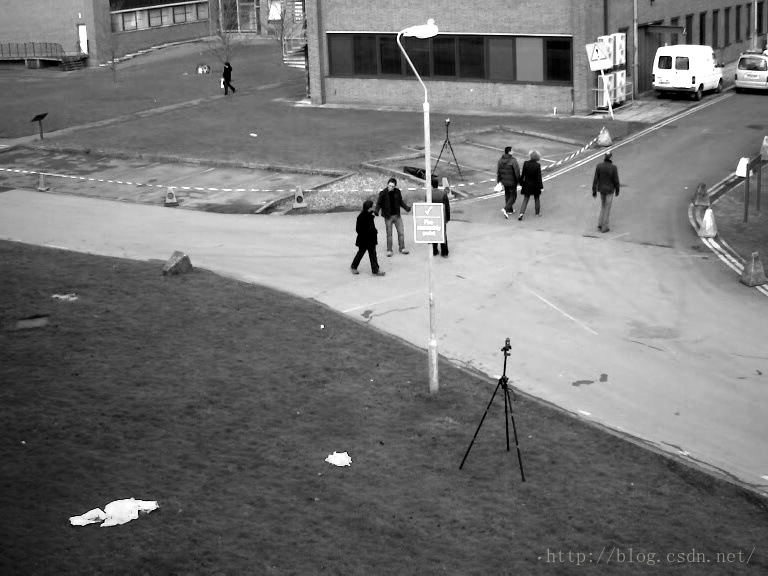
\includegraphics[width=0.45\textwidth]{pictures/6lap1} %插入图片命令,格式为[配置]{图片路径}
    }
    \quad %空格
    \subfloat[]{
	\label{Fig:R2} % 子图2标签名
    	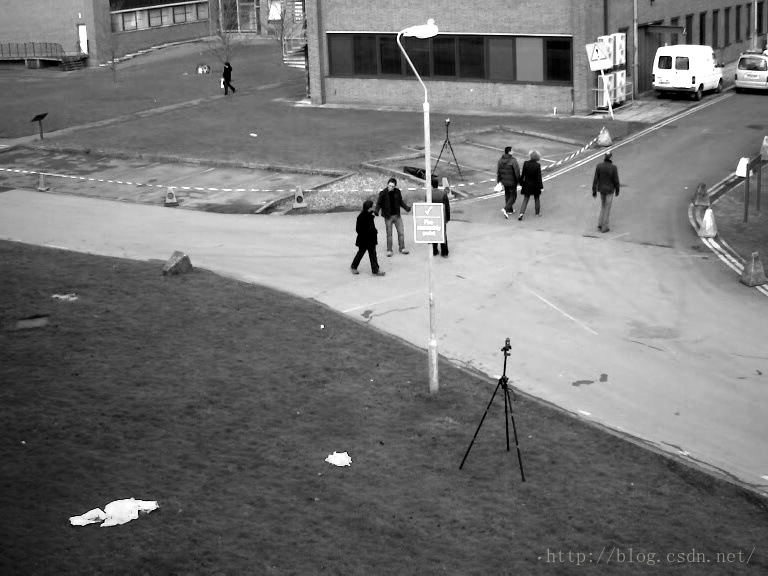
\includegraphics[width=0.45\textwidth]{pictures/6lap1}
    }
   \caption{相邻帧间差分法原图} %注意须使用\protect\subref{}进行标号引用
    \label{Fig:6lap} % 整个组图的标签名


\end{figure}

\buptfigure[width=0.7\textwidth]{pictures/6lap2}{相邻帧间差分法差分图}{6lap2}

\subsection{高浮动区域检测}
	对于本课题的定位数据,帧间差分法所实现的功能即是检测出由于异常导致的子区域定位数据的剧烈抖动。由于台风过境这类异常事件的产生,使得图中某一部分的定位数据相较于正常数据产生较大的变化,这些变化可以使定位数据产生的图像之间差分后在图中明显观察得到,之后再用滑动窗的方法去检测具体区域。
	正常情况下的数据帧间差分效果如图\ref{6normal}所示:

\buptfigure[width=0.9\textwidth]{pictures/6normal}{正常定位数据间相邻帧差分图}{6normal}

	在第5章中我们检测出9月30日午间的定位数据存在异常,我们将其与9月29日的同时刻数据进行帧间差分,如图\ref{6errorwithout}所示:

\buptfigure[width=0.9\textwidth]{pictures/6errorwithout}{异常与正常定位数据间相邻帧差分图}{6errorwithout}

	由图可见,存在异常的时刻与正常时刻的定位数据图进行差分会在图中看到明显的“亮”区域,即变化幅值较大。我们再使用滑动窗的方法去检测高浮动区域,使用不同大小的正方形滑动窗对整个范围内进行搜索,自动标记出几个平均密度最高且超过阈值的区域,在图\ref{6error}中显示如下:

\buptfigure[width=0.9\textwidth]{pictures/6error}{异常与正常定位数据间相邻帧差分图}{6error}

	图中所标记的异常浮动值主要集中在城市区域,由于9月30日是国庆节前一天,可能是游客的集中所造成的定位数据量增大。 

\chapter{总结与展望}


\section{内容总结}
	现代科学的发展,使得传感器网络越来越普及,让大数据分析成为可能。在这些数据之中,有一种数据尤为重要,其存在着很明显的时序性,描述着随着时间的推进中,某种事物的变化规律,这种数据常被称为时序数据。时序数据分析是对时间序列进行系统的分析并且简历合理的模型。其主要目的是考虑数据动态的波动情况并预报未来发生的事件。本文所讨论的定位数据就是基于某固定的空间坐标上的时序数据点,通过这种定位数据的时序分析,可以归纳总结出该地的人流变化特征。而对于存在明显规律的时序数据,我们可以对其进行建模并预测当前或未来时间节点上的值。
	但是,时序数据中经常会出现这样一些的观测点,它们的数据值较同性质时段上的数据存在着明显的偏差,我们称其为异常点。异常点的分析以及处理十分有意义:一方面异常点对于时间序列的建模来说是干扰很严重的噪音,较大的异常会使得拟合模型造成极大的偏差,需要将这些异常点检出并且删去使得模型的训练及预测更加精准;而另一方面,时序定位数据中的异常又反应出了该时间点上一定存在着某种外界干扰,比如定位数据急剧降低可能是由于台风过境人群大量躲在遮蔽物处而造成的。对于台风这种自然灾害,如果能根据时序定位数据的预测以及异常的判断,则能很好的做好预警,显得尤为重要。本文根据以上思路,基于腾讯的定位数据,对时序异常检测及相关内容完成了以下工作:
\begin{enumerate}
\item \textbf{数据分析}:对给定的腾讯定位数据进行处理后有了其基本的背景信息,以及为了后续的分析方便进行了预处理。给定的腾讯定位数据大致地理坐标为广东省珠海市沿海一带,而明确探查出的异常是某天的台风过境;由于地图上涵盖一大部分海面,而海面上的定位数据(定位终端数量)几乎为零,分析这些数据毫无意义,故通过最大值判断的方法进行了舍去;最后,通过数据的可视化,以及考虑到存在部分局部时刻异常的情况,我们得出了通过分析每天定位数据平均值来反应整天的定位数据信息,并统计分析图中所有地理坐标上的定位数据信息来确定某天是否存在异常的结论。
\item \textbf{基于曲线的异常检测分析}:我们将原本的整块区域异常天检测问题(本课题的异常为台风日)细化为各个有效定位数据点在数据范围日期内的一条曲线,并对整个定位数据点区域的每个点做曲线分析并统计结果;在曲线分析中,我们使用了基于统计、密度、差分、频域的几种曲线分析方法去检测异常并都成功将异常日期找出;最后,基于本课题的定位数据,我们分析了曲线异常检测的几种算法的特点并且讨论了本算法的局限性。
\item \textbf{基于曲线的时序数据预测}:由于前述曲线异常检测的算法对于检出局部时刻异常较为困难,我们采用预测并比较的方法去检测异常。神经网络能够经过数据的训练来对网络结构中的参数进行调整,从而使网络近似趋近于时间序列的实际规律;我们对本课题所研究的腾讯时序定位数据中一部分进行了训练,使用该预测模型对国庆前的某一小时时刻的定位数据进行了预测及判断,预测与实际值有较大偏差,可以检出局部时刻的异常。
\item \textbf{基于图像的异常区域检测}:本章基于上述两章的检测结果,研究在检测区域中哪一块小区域出现了大浮动从而导致了异常;使用了图像相邻帧间差分法,观察到异常时刻与正常时刻的定位数据差分图较正常时刻之间的差分图颜色更深,并使用了不同大小的矩形窗计算差分定位数据图中平均异常变化幅度,将最大的几块区域圈出。
\end{enumerate}

\section{未来展望}
本文的实验表明,在基于腾讯地图的时序定位数据上,我们能够成功检出已知的台风天异常并建立预测模型达到实时异常检测的目的,并且能够根据异常的时间点找出异常子区域。但对于实际定位数据的分析来说,本文在以下方面可以进行改善:
\begin{enumerate}
\item \textbf{高地理精度定位数据的异常检测}:本文所研究的课题所涉及的定位数据是大区域的粗精度数据,一个像素点约代表平方一千米以上的量级,算法对于分析大范围内的整体异常是有效的。但实际情况中有时研究者所接触到的定位数据是更高精度的,此时本文所讨论的对于整体区域的异常检测不再有效,高精度下应该更关注地理位置上的部分区域,应做更进一步探索。另外,本文对数据所做的简化处理也无法再适用于高精度的数据,无论是时空上或是地理上高精度的定位数据有更多信息可以挖掘,无法直接从统计角度进行整体分析,应当对数据进行更加细致的分析研究可实现的算法。
\item \textbf{大规模数据的曲线异常检测}:本文所实现的曲线异常检测算法中,部分算法对于本课题所研究的小规模数据量表现不佳,例如极大似然估计法这类统计方法,当数据量足够大时可能会把数据模型的参数拟合的较好,从而能更好地判断数据是否异常。同样,对于第5章所讨论的神经网络时序数据预测,数据量小时可能会导致网络模型拟合不佳,对于数据的拓展预测不利。
\item \textbf{异常值偏离正常值的门限}:本文所实现的曲线异常检测算法中,尤其是根据对已知的台风异常检测,设定了一个固定的门限来判断是否存在异常。实际情况中,定位数据会根据各种外在因素导致偏差,无法断定异常的偏差值设为多少才合适。应当具体问题具体分析,对当地的数据有一个大规模的统计,才能划定出最适合该地的异常值门限。
\end{enumerate}



%%%%%%%%%%%%%%%%%%%%%%% Main Area ENDs Here %%%%%%%%%%%%%%%%%%%%%%%%
%\let\cleardoublepage=\cleardoublepagebak
% Reference
\clearpage\phantomsection\addcontentsline{toc}{chapter}{参考文献}
\bibliographystyle{buptbachelor}
\refbodyfont{\bibliography{ref}}

% Thanks to page
\clearpage\phantomsection\addcontentsline{toc}{chapter}{致\qquad{}谢}
\chapter*{致\qquad{}谢}
\normalsize\thankwords

% Appendix
\setcounter{figure}{0} 
\renewcommand{\thefigure}{~附-\arabic{figure}~}
\setcounter{equation}{0} 
\renewcommand{\theequation}{~附-\arabic{equation}~}
\setcounter{table}{0} 
\renewcommand{\thetable}{~附-\arabic{table}~}

\chapter*{附\qquad{}录}
\phantomsection\addcontentsline{toc}{chapter}{附\qquad{}录}

\phantomsection
\addcontentsline{toc}{section}{附录1\quad{}缩略语表}
\section*{附录1\quad{}缩略语表}

\begin{bupttable}{定位数据相关名词解释}{crowdwisdom}
    \begin{tabular}{l|l|l}
		\hline \textbf{特征} & \textbf{描述} & \textbf{形式与理论范围}\\
		\hline 定位数据值 & 确定地理坐标在某时刻检测到多少定位终端数量 & 数值,$\mathbb{N}$ \\
		\hline 时序定位数据值 & 确定地理坐标在离散时间区间内各时刻的定位数据值 & 数组,$\mathbb{N}$ \\
		\hline
    \end{tabular}
\end{bupttable}


\phantomsection
\addcontentsline{toc}{section}{附录2\quad{}数学符号}
\section*{附录2\quad{}数学符号}
\begin{center}
	\begin{tabular}{ccc}
		\multicolumn{2}{c}{\textbf{数和数组}} \\
		\\
		$a$ & 标量(整数或实数)\\
		$\bm{a}$ & 向量\\
		$\bm{t_a}$ & a时刻\\
		$\bm{x_a}$ & a时刻的定位数据值\\
		$\bm{d_a}$ & a时刻的定位数据值与相邻时刻值间差分\\


	\end{tabular}
\end{center}

\newpage\backmatter
% Translation
\chapter*{外\quad{}文\quad{}译\quad{}文}
\vspace{8mm}

\thispagestyle{empty}

\begin{center}
\sihao\heiti{Yahoo大规模时列数据异常检测技术及其高性能可伸缩架构}

\xiaosihao\songti{Nikolay Laptev, Saeed Amizadeh, Ian Flint}

\xiaosihao\songti{Yahoo Labs}
\end{center}

\songti{}
\let\clearpage\relax

%以下是排版示例,在这里为了使章节编号不出现在目录中,使用了无编号的样式,代价是这些数字都要自己书写。另外,由于外文文献一般不是很长,为了排版紧凑,每一章被设置为不另起一页。

\chapter*{摘要}
本文介绍了一种用于大规模时序数据自动异常检测的通用和可扩展框架。及早发现异常情况对维护个人数据的一致性和保护公司免受恶意攻击者起着关键作用。目前最先进的异常检测方法受可扩展性,用例限制,使用困难和大量误报的影响。我们在雅虎(EGADS)的系统设计了基于异常检测和预测模型构建的异常过滤层,以实现时序精确和可扩展的异常检测。我们将我们的方法与具有不同时间序列特征的真实和合成数据的其他异常检测系统进行比较。我们发现,我们的框架可以使各种用例的精度和召回率提高50-60%,并且数据和框架都是开源的。


\chapter*{第一章\ 概述}
虽然计算硬件和软件方面的快速发展带来了强大可靠的应用程序,但仍然有数百个软件错误和硬件故障在大型集群中继续发生,从而影响用户体验并随后恢复。不间断系统具有严格的正常运行时间要求,对这些系统的持续监控至关重要。从数据分析的角度来看,这意味着不停地监测大量的时间序列数据,以便检测潜在的故障或异常情况。由于问题的规模很大,人们对这些数据的监测实际上是不可行的,这导致我们使用机器学习和数据挖掘技术进行自动异常检测。

异常或异常值是与其余数据显着不同的数据点。一般来说,大多数应用程序中的数据是由一个或多个反映系统功能的生成过程创建的。当潜在的生成过程以不正常的方式运行时,会产生异常值。对这些异常值进行快速有效的识别对于许多应用非常有用,这些应用包括:侵入检测,信用卡欺诈,传感器事件,医疗诊断,执法等。
自动化异常检测中的现有方法源于大量误报,这些误报在实践中禁止了这些系统的实用性。用例或类别特定的异常检测模型,可能对特定应用程序的误报率较低,但当时间序列的特征发生变化时,这些技术在没有适当的再训练的情况下表现不佳。第6.3节在实践中证明了“一刀切”原则的缺陷。
我们在雅虎的系统被称为EGADS(可扩展通用异常检测系统),它可以准确,可扩展地检测时间序列异常。 EGADS将预测,异常检测和警报分为三个独立的组件,允许用户将自己的模型添加到任何组件中。
EGADS使用一组经过调整的默认模型来减少误报数量,这对于普通用户来说本身就足够了。然而,更高级的用例需要系统捕获某些类型的异常,而忽略其他异常。值得引起注意的异常可能在幅度,严重程度或其他未知的先验参数上有所不同,并取决于用例。为此,EGADS的警报组件使用机器学习为消费者选择最相关的异常情况。
EGADS是首个灵活、准确且可扩展的异常检测综合系统。 EGADS框架与异常检测基准数据已经一同开源,旨在帮助学者和行业合作开发新的异常检测模型。在雅虎,EGADS每天被许多团队用于数百万次的时间序列异常检测工作。
在第2部分中,我们描述了EGADS体系结构。算法和警报模块分别在第3节和第4节中介绍。以前的工作将在第5节中介绍。实验将在第6节中讨论,然后分别讨论第7节和第8节中的实际用例和结论。

\chapter*{第二章\ 整体架构}
GADS框架由三个主要部分组成:时间序列建模模块(TMM)、异常检测模块(ADM)和报警模块(AM)。给定一个时间序列,TMM组件模拟产生时间序列,由ADM和AM组件进行消费处理,分别计算误差并过滤不感兴趣的异常。这些组件在第3和4节中有详细描述。

EGADS被构建为一个框架,可以轻松地集成到现有的监控基础设施中。在雅虎,我们内部的雅虎监控服务(YMS)每秒处理数百万个数据点。因此,对YMS进行可扩展、精准且自动化的异常检测至关重要。接下来我们将详细描述YMS的具体细节。

\section*{2.1\ 系统集成}
EGADS作为独立平台运行,可用作大型系统中的库。因此,设计EGADS和雅虎监控服务(YMS)之间的接口至关重要。 EGADS与YMS的集成架构图如图\ref{f1}所示。

\buptfigure[width=0.7\textwidth]{pictures/f1}{EGADS-YMS 整体架构}{f1}

此外,异常检测还需要几个支撑组件来驱动完成。首先,所有的异常检测模型都是离线批处理(batch)产生的,然后应用到实时环境(real time)。其中批处理由三个步骤组成:

\begin{enumerate}
\item 监测数据(即监控的时间序列数据)批量存储在Hadoop集群上
\item 批量模型生成器针对这些数据运行,并为目标时间序列构建模型
\item 模型存储在模型数据库中
\end{enumerate}

然后在线实时流使用这些存储的模型,具体步骤如下:

\begin{enumerate}
\item 数据流入Storm进行流式处理
\item 集群中的一个模块调用EGADS ADM,根据存储在模型数据库中的模型来评估输入数据点
\item 如果存在异常,则将其发送到由组合规则和其他包含特定逻辑组成的辅助规则流(见第4节)
\item 根据规则,如果异常是警报事件,则生成事件,存储在状态数据库中,并转发到警报路由系统
\item 警报路由系统应用路由配置规则将警报发送给相应的处理人员
\end{enumerate}

\section*{2.2\ 可拓展性}
	EGADS的监控需要每秒分析超过百万级数据点和亿级别时间序列。要求在CPU负载、I/O和内存占用方面具有可扩展性,并且数据点的处理需要尽可能高效。这意味着需要预先计算尽可能多的模型。从磁盘读取模型是不切实际的,会降低性能,因此模型应该存储在内存中。另一方面,为了控制成本,模型应尽可能小。


\chapter*{第三章\ 异常检测算法}
	在本节中,我们给出了EGADS支持的异常检测算法。目前,EGADS能够检测出三类异常:

\begin{itemize}
\item \textbf{异常值}:给定输入时间序列x,异常值为时间戳值对$\bm{t,x_t}$,其中观察值xt与此时的时间序列的期望值显着不同,即$\bm{E(x_t)}$。
\item \textbf{波动点}:在给定输入时间序列$\bm{x}$的情况下,变化点是在时间戳$\bm{t}$上,使得时间序列的行为在$\bm{t}$之前和之后显着不同。
\item \textbf{异常时间序列}:给定一组时间序列$\bm{X = \{x^i\}}$,异常时间序列$\bm{x^j\in X}$是在$\bm{X}$上与大多数时间序列不一致的部分。
\end{itemize}

在以下章节中,我们给出了EGADS当前用于检测上述异常类型的方法。

\section*{3.1\ 异常检测}

检测异常值是许多监控应用中最重要的功能。EGADS提供了两类用于检测输出的算法,本节对这两类算法进行了描述。

\subsection*{3.1.1\ 插件方法}
	EGADS中异常值检测的第一类方法称为插件方法。为了模拟输入时间序列的正常行为,可以业务和时序数据的特点来插入大量的时间序列模型和预测模型(例如ARIMA、指数平滑、Kalman滤波、状态空间模型等)。这就是为什么我们将这个总体策略称为插件方法。应该注意的是,所有这些模型都在EGADS中用于时间序列预测,这是我们框架的另一个特征;然而,由于本文的重点是异常检测,更多关于EGADS的建模和预测特征的细节我们不进行更深入的讨论。

	我们提出的Plug-in框架包含两个主要组件:时间序列建模模块(TMM)和异常检测模块(ADM)。给定时间序列$\bm{X=\{x_t\in R:\forall t\ge 0\}}$,TMM提供在时间$\bm{t}$的$\bm{x_t}$的预测值,用$\bm{u_t}$表示。我们也把这个数量称为$\bm{x_t}$的期望值(不要与期望的数学概念混淆)。 TMM可以是预测的机器学习模型,基于一些训练数据或基于规则的系统,在时间$\bm{t}$上挖掘数据点$\bm{x_t}$的具体表现特征(如波动或异常)。在本文中,我们不对TMM做任何假设;也就是说,TMM只是我们提出的生成预测的方法中的一个黑盒模块。从这个意义上说,我们提出的框架是通用的,并不依赖于任何特定的时间序列建模框架。

	给定预测值$\bm{u_t}$和实际观测值$\bm{x_t}$,ADM计算出一些我们称之为偏差度量(DM)的偏差概念。最简单的偏差量度是预测误差,即

	$$\bm{PE_t=x_t-u_t}$$

如果错误超出某些固定阈值,则会发出警报。这种简单的方法在某些情况下可能会起作用,但是对于大多数的方法来说,它不会是一个很好的策略,因为它不能捕获到错误的具体信息。相对误差$\bm{RE_t}$被定义为$\bm{u_t}$的一个因素:

	$$\bm{RE_t=\frac{x_t-u_t}{u_t}=\frac{x_t}{u_t}}$$

通过对相对误差进行阈值处理,可以检测异常值,同时对所期望值的幅度进行归一化。虽然这些阈值确定了异常检测模块的敏感度,然而,很难确定异常检测的最佳度量。事实上,给定时间序列的最优度量的选择取决于时间序列的性质以及TMM性能。例如,如果我们处理一个非常规则的时间序列,我们有一个准确的模型,使用预测误差进行异常检测可能就足够了,因为它预期是正态分布的。在其他情况下,最佳度量可能在预测误差和相对误差之间存在某种差异。因此,EGADS默认跟踪一组偏差度量,使用系统的人可以创建自己的错误度量。在第4节中描述的警报模块(AM)中使用这些错误度量以及其他功能(如时间序列特征)来了解用户的偏好并过滤不重要的异常。

\subsection*{3.1.2\ 基于分解的方法}

EGADS中第二类异常值检测方法是基于时间序列分解的思想,在时间序列分析中,通常将时间序列分解为:趋势、季节性和噪声三个要素。通过监测噪声分量,可以捕获异常值。更准确地说,如果点Xt的噪声分量的绝对值大于某个阈值,则可以认为Xt为异常值。

\section*{3.2\ 变点检测}

在一些文献里有提到一种基于时间窗口的变点检测技术,在EGADS中,目前采用基于模型的方法。在这些方法中,时间序列的预期行为通过3.1.1节中提到的建模技术建模。我们结合3.1.1节中描述的插件方法来计算输入时间序列的残差序列(或模型预测的偏差)。然后我们对残差序列应用绝对变化点检测的方法来检测残差分布。我们使用内核密度估计(Kernel Density Estimation)、非参数估计残差分布和Kullback-Leibler(KL距离,常用来衡量两个概率分布的距离)来测量分布变化。

\section*{3.3\ 检测异常时间序列}

EGADS支持的另一类异常检测技术涉及检测异常时间序列。异常时间序列$\bm{t}$被定义为与其他时间序列的平均偏差显着的时间序列。假设所有时间序列是均匀的并且来自相同的来源(即,是同一个群集的一部分),可以简单地计算相对于其他时间序列的时间序列$\bm{(i)}$的平均偏差。在EGADS中,我们目前的方法是根据各种时间序列特征(包括趋势和季节性,谱熵,自相关,平均欧几里德距离等)将时间序列聚类为一组聚类$\bm{C}$。在聚类后,我们执行簇内或簇间通过测量聚类质心和时间序列$\bm{(i)}$内部或之间的偏差来进行时间序列异常检测。这种EGADS异常检测类型的常见用例涉及分类。例如,如果网络工程师想要在数百万个时间序列中找到异常服务器,对于以前的方法来说可能是不切实际的,因为建模是按照时间序列来完成的,而不考虑其他度量的行为。这种异常检测类型的另一个应用是发现类似的异常,这与以前的用例相反。

\chapter*{第四章\ 警报机制}
异常检测的最终目标是产生准确和及时的警报。 EGADS通过两阶段过程实现这一点,首先通过阈值选择产生一组候选异常,然后根据给定的规则过滤不相关的异常。

\section*{4.1\ 阈值选择}
阈值选择的作用是根据异常检测模块(ADM)产生的偏差度量选择合适的阈值。目前,EGADS基于以下两种阈值选择算法实现:
\begin{itemize}
\item $\bm{K\sigma}$偏差
\item 密度分布
\end{itemize}

第一种方法是参数化的,并假定数据正态分布,有明确的平均值和标准偏差。依靠高斯分布,并基于“3sigma规则”(即:其中99.73%的样本位于平均值的三个标准偏差之内)。因此,根据Kσ中的K值,可以确定在时间t观测样品的可能性。根据所需的敏感度,可以测量给定的样品是否在K = 2或1的所有样品的95.45%或68.27%之内。请注意,这里的假设是以我们的偏差度量是正态分布为前提的。 第二种方法是非参数的,对于偏差度量不是正态分布的情况是有用的。基本思想是找到偏差度量分布的低密度区域。一种方法是使用诸如局部离群因子(LOF)的算法。通过将对象的局部密度与其邻居的局部密度进行比较,可以识别具有相似密度的区域,以及具有比邻居密度明显更低的密度的点,这些点被认为是异常值。

\begin{bupttable}{EGADS所使用的时序数据特征表}{t1}
    \begin{tabular}{l|l}
		\hline \textbf{时间序列功能} & \textbf{描述} \\
		\hline 周期(频率) & 周期性对于确定季节性非常重要。 \\
		\hline 趋势 & 如果平均水平有长期变化,则其存在  \\
		\hline 季节性 & 时间序列受季节因素影响时存在,例如一年的月份或一周中的某一天  \\
		\hline 自相关 & 代表长期依赖。\\
		\hline 非线性 & 非线性时间序列包含通常不由线性模型表示的复杂动态。  \\
		\hline 偏态 & 衡量对称性,或者更确切地说,缺乏对称性  \\
		\hline 峰度 & 相对于正态分布来衡量数据是否达到峰值或持平。\\
		\hline Hurst & 衡量时间序列的长期记忆。 \\
		\hline Lyapunov 指数 & 衡量附近轨迹发散率的指标。 \\
		\hline
    \end{tabular}
\end{bupttable}

\section*{4.2\ 过滤}

过滤对异常进行最后阶段的后期处理,然后交付给消费者。虽然作为过滤阶段输入的候选异常具有统计意义,但并不是所有这些异常都会与特定用例相关。例如,一些消费者对时间序列中的峰值感兴趣,而其他消费者对下点感兴趣,而其他消费者则对变化点感兴趣。 EGADS提供了一个简单直观的界面,允许用户标记异常时间序列的区域。 EGADS将此反馈与时间序列和模型特征一起用于训练预测异常ai是否与用户uj相关的分类器。 EGADS跟踪的时间序列特征见表\ref{42}。在第6.2节中,我们将看看这些时间序列特征如何影响模型性能。

\buptfigure[width=0.7\textwidth]{pictures/f2}{EGADS提取的时间序列及其特征的一个示例}{f2}

\chapter*{第六章\ 实验研究}

\section*{6.1\ 数据}
用于实验的数据集由1:1的合成数据和真实数据混合而成。我们创建了一个合成的时间序列生成工具,该工具已经随着框架和基准数据开源。使用该工具,通过指定长度、幅度、异常数、异常类型、异常大小、噪声水平、趋势和季节性来生成合成时间序列。真实数据集使用了雅虎会员登录数据(YML)。合成和真实数据在时间序列都包含3000个数据点,YML数据包含了3个月的数据点。除非另有说明,所有实验均以1000次随机选取的时间序列进行,结果取平均值。还要注意,合成和真实数据都有异常标签,方便测量精度和召回率。

\section*{6.2\ 建模实验}
时间序列建模(由EGADS中的TMM组件捕获)是异常检测的基本部分。通常情况下,异常检测与底层时间序列模型一样好。由于大量的候选模型,模型选择变得至关重要,并且取决于时间序列特征和可用资源。在下面的实验中,我们展示了时间序列特征对模型性能的影响,并显示了精度,实验中使用的模型和误差度量分别参见表\ref{t2}和\ref{t3}。

\begin{bupttable}{用于建模实验的模型列表}{t2}
    \begin{tabular}{l|l}
		\hline \textbf{模型} & \textbf{描述} \\
		\hline Olympic Model & 朴素的季节模型,其中下一点的预测是前n个周期的平滑平均值。 \\
		\hline 指数平滑模型 & 一种流行的模型,用于生成平滑的时间序列。  \\
		\hline 移动平滑模型 & 在这种模式下,预测基于一个人为地构建的时间序列。  \\
		\hline 回归模型 & 使用一个或多个变量来怼x和y之间的关系进行建模。\\
		\hline ARIMA & 自回归整体移动平均线。  \\
		\hline (T)BATS系列 & (三角函数)指数平滑状态空间模型与Box-Cox变换。  \\
		\hline Kalman谱滤波器 & 一个内部算法用于学习卡尔曼滤波器参数的快速多变量谱。  \\
		\hline
    \end{tabular}
\end{bupttable}

\begin{bupttable}{用于建模实验的指标列表}{t3}
    \begin{tabular}{l|l}
		\hline \textbf{指标} & \textbf{描述} \\
		\hline Bias & 误差的算术平均值 \\
		\hline MAD & 平均绝对偏差  \\
		\hline MAPE & 平均绝对百分比误差  \\
		\hline MSE & 误差的均方\\
		\hline SAE & 绝对误差的总和  \\
		\hline ME & 平均误差  \\
		\hline MASE & 平均绝对比例误差  \\
		\hline MPE & 平均百分比误差  \\
		\hline
    \end{tabular}
\end{bupttable}

\subsection*{6.2.1\ 时间序列特征和性能}
为了证明时间序列特征对模型性能的影响,我们比较了不同模型的时间序列与不同特征的误差度量(见4.2节)。图\ref{f3}显示了时间序列特征在模型行为中起着重要作用。例如,季节性模式的Olympic模型在数据集上表现不佳,没有季节性和强劲趋势。 EGADS能够跟踪历史时间序列特征和模型性能,使用这些历史信息,EGADS选择由表3中描述的误差度量判断的最佳模型(给定时间序列特征)。实际上,基于数据特征进行模型选择比针对每个模型执行交叉验证要快得多。

\buptfigure[width=0.7\textwidth]{pictures/f3}{具有不同特性的时间序列性能}{f3}

\subsection*{6.2.2\ 时序模型的可扩展性}
如第2节所述,时序模型需要高性能技术以支持大规模(例如每秒数百万点)数据流的实时计算,因此需要在模型大小、训练时间和准确性之间进行权衡。 这种权衡在图\ref{f4}(a)和(b)中可以看出。 例如,从图中可以看出,季节性天性模型训练很快,但是具有较大的存储要求和较高的平均误差。 在雅虎,首先设定了资源和模型训练时间的目标,然后选择相应的模型。 换句话说,目标是在资源和模型建立时间限制下使得表3中的错误减到最小。

\buptfigure[width=0.7\textwidth]{pictures/f4}{模型大小与训练时间的权衡}{f4}

\section*{6.3\ 异常检测实验}
在本节中,我们比较了开源系统与EGADS,参考的开源系统如表\ref{t4}所示

\begin{bupttable}{建模实验的指标列表}{t3}
    \begin{tabular}{l|l}
		\hline \textbf{模型} & \textbf{描述} \\
		\hline EGADS Extremelow 密度模型异常值 & EGADS基于密度的异常检测 \\
		\hline EGADS CP & 基于EGADS内核的波动点检测  \\
		\hline EGADS KSigmaModel异常值 & EGADS重新实现了经典的$\bm{K\sigma}$模型  \\
		\hline Twitter Outlier & 基于广义ESD方法的开源Twitter-R异常检测库\\
		\hline Extreme\&II R异常值 & 开源单变异常值检测,阈值绝对值和残差检测异常  \\
		\hline Breakout Twitter CP & 来自Twitter基于ESD统计测试来检测变化点的一个库  \\
		\hline ChangePt1 R CP & 一个R库 ,实现各种主流和专门的变化点方法\\ 
		\hline ChangePt2\&3 R CP & 检测平均值和变量的变化  \\
		\hline
    \end{tabular}
\end{bupttable}

在图\ref{f5}显示了对6.1节中描述的数据的测试结果:

\buptfigure[width=0.7\textwidth]{pictures/f5}{异常模型在不同数据集上的表现}{f5}

结果可以看出,没有一个最佳的异常检测模型能适合所有业务场景,不同的算法需要结合检测不同类型的异常来确定。例如,Twitter在数据集上表现最好,而ExtremeLowDensity模型在上表现最好。但是,EGADS的设计初衷是在用户对数据类型的时间序列和异常类型不了解的情况下,该系统能够优雅和稳健地处理数据中存在的各种异常现象。因此,EGADS被构建为将一组异常检测模型组合成一个最佳框架的库。这些模型的异常被转发到过滤组件以进行精确的异常检测。

\section*{6.4\ 异常过滤实验}

异常的重要性往往取决于实际应用场景。具体来说,一些用户可能对展示恶意攻击的时间序列行为感兴趣,而其他用户可能对收入有兴趣。

为了解决这个要求,过滤阶段扫描所有模型的所有异常,并使用分类为作为真正的模型。在YM用例的过滤阶段使用的模型是基于AdBoost的增强树模型。模型中使用的特征参见表\ref{t1}。AdaBoost的核心原理是在变化的数据上进行适合一系列weak learners(例如,小决策树),最后的结果是通过组合加权多数表决产生的。图6中的实验结果表明,在滤波阶段使用不同的模型特征,得到比较好的精确率和召回率。

\buptfigure[width=0.7\textwidth]{pictures/f6}{使用不同类型特征的过滤阶段的精度}{f6}

\chapter*{第七章\ Yahoo实例应用}

\section*{7.1\ 系统度量}
系统指标广泛地定义为服务系统中硬件组件的健康状况的度量。 例子包括CPU利用率,可用磁盘空间,网络接口流量统计和内存利用率。 其中一些度量标准(如CPU利用率)跟踪组件的总体流量,一些(如可用磁盘空间)与当前流量级别无关。 系统指标与其他类型的指标不同之处在于,由于雅虎服务系统的冗余特性,阈值违反通常是服务问题的主要指标。 因此,针对这些类型的指标的警报通常不会被视为中断,而是用于触发长期补救措施,如添加容量或清除磁盘空间。

\section*{7.2\ 业务绩效}
业务KPI是直接反映客户与雅虎网站体验的指标。 示例包括页面浏览量,服务延迟时间,服务错误,点击率和收入等。 业务KPI几乎总是网站问题的尾随指标,定义反映了对雅虎服务能力的影响。 因此,业务关键绩效指标的异常情况通常都会受到高度的关注。 大规模业务关键绩效指标的性质是它们往往具有高度的可预测性,所以它们很适合自动化异常检测。 雅虎在整合业务KPI方面取得了巨大成功,可通过自动化异常检测发现服务和收入问题。

\section*{7.3\ 相似度量组}
雅虎的大部分基础架构都遵循横向扩展模型,每个服务层都有数十台到数百台服务器。 在对可疑事件的原因进行分类和隔离时,可能很难调查数千台机器的基础设施以发现故障。 自动异常检测可用于对基础设施各组成部分的相对异常情况或“兴趣度”进行排序,这些特征可按降序排列,以便操作员能够快速查看模式并隔离问题。


\chapter*{第八章\ 总结}
异常检测是许多具有故障应用的实时监控系统的核心部分, 比如检测、欺诈检测、网络入侵检测等等。尽管它至关重要,但实际上实施全自动异常检测系统是一项极具挑战性的任务,这些挑战通常导致解决方案不可扩展或并非高度专业化的,也导致了较高的误报率。

在本文中,我们介绍了EGADS——雅虎实现的通用异常检测系统,对不同的Yahoo属性和数百万个时间序列进行自动监控和警报。正如我们在本文中所描述的,Hadoop上的EGADS并行架构以及Storm的流处理机制使得它能够在雅虎的数百万个时序数据集上执行实时异常检测。此外,EGADS采用不同的时间序列建模和异常检测算法来处理不同的监控场景。通过将这一组算法与机器学习机制结合到警报模块中,EGADS能自动适应对用户重要的异常检测用例。所有这些功能都有效地创建了一个功能强大的异常检测框架,它是通用且可扩展的。我们对真实数据集和综合数据集的展示实验表明,与其竞争对手的解决方案相比,我们的框架具有优越的适用性。

EGADS的设计本质上是可扩展的,它为向系统插入新的模型和算法提供了一种简单的机制。我们的框架及其所有数据集都已经开源。
% Translated Article
\thispagestyle{empty}
\begin{center}
% 原文第一页,PDF缩放比例为0.95,可以自行调整
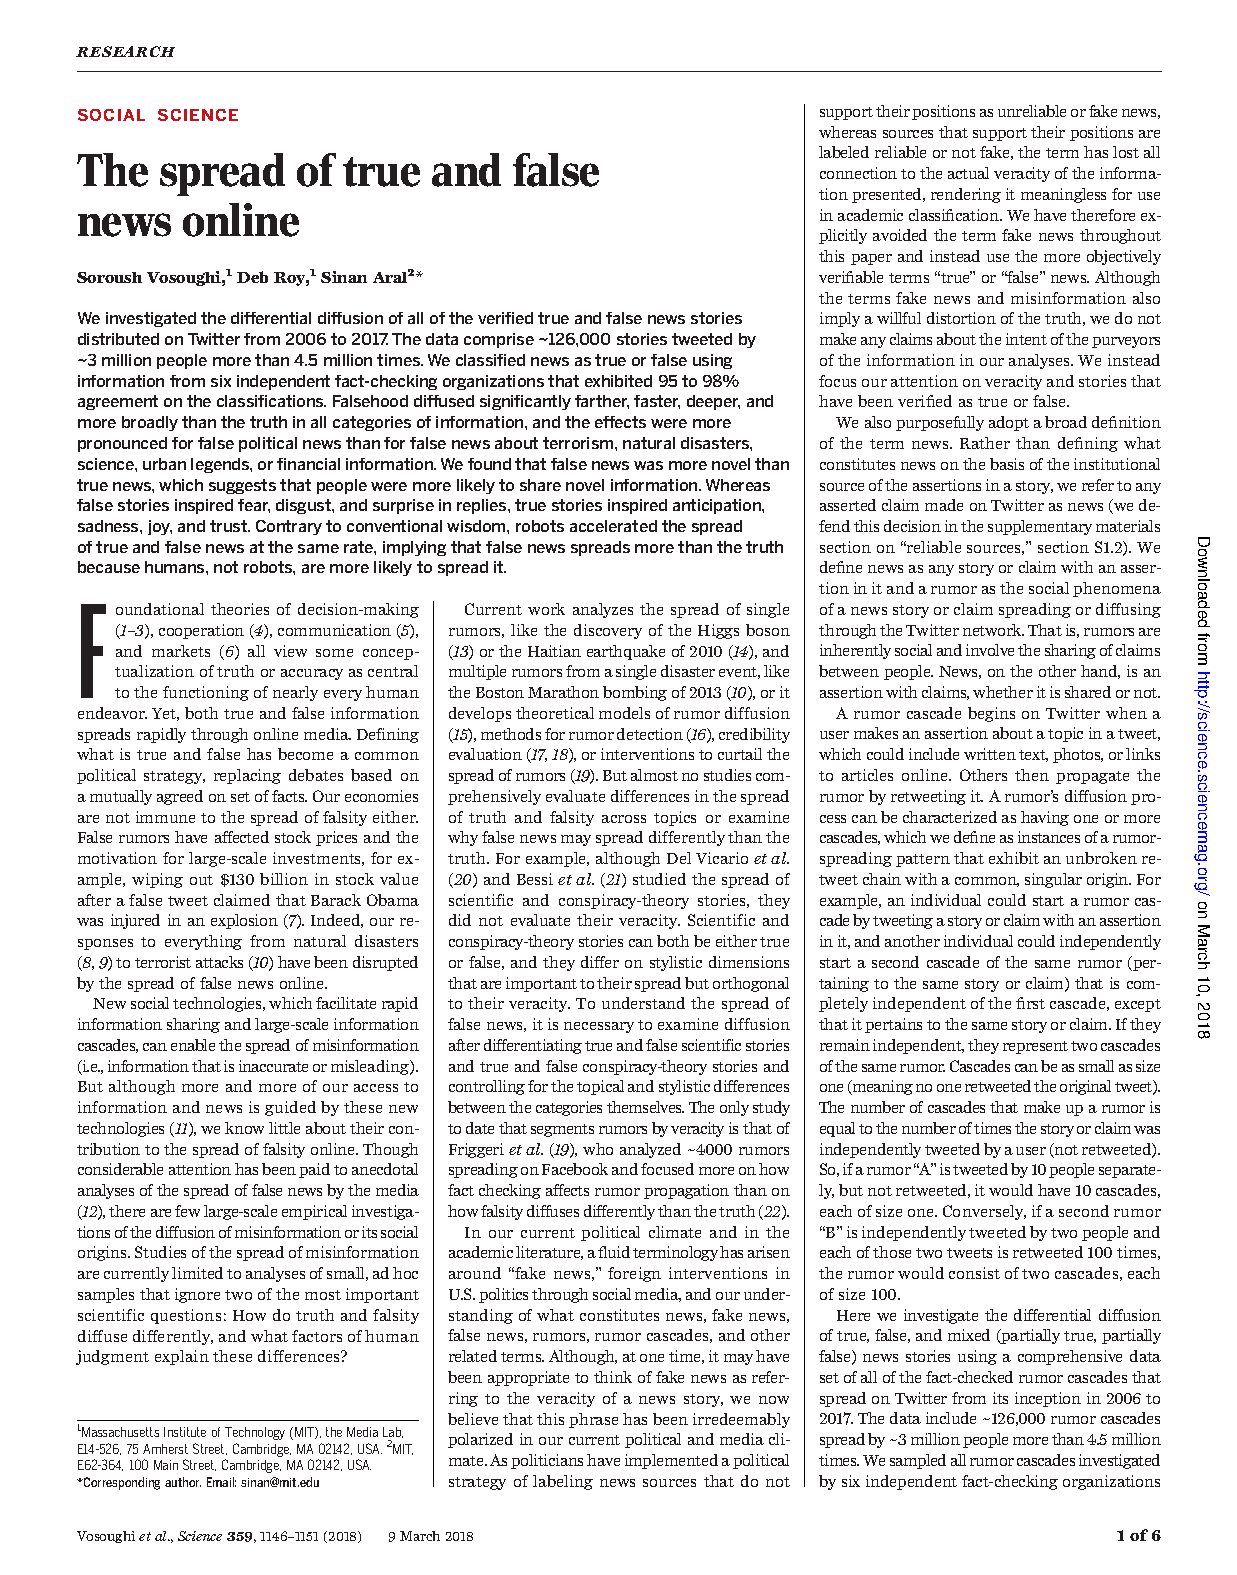
\includepdf[pages=1, scale=0.95, pagecommand=\heiti\sanhao{\textbf{外\quad{}文\quad{}原\quad{}文}}]{docs/translation.pdf}
% 原文剩余部分
\includepdf[pages=2-, scale=0.95, pagecommand={}]{docs/translation.pdf}
\end{center}

% 开题报告
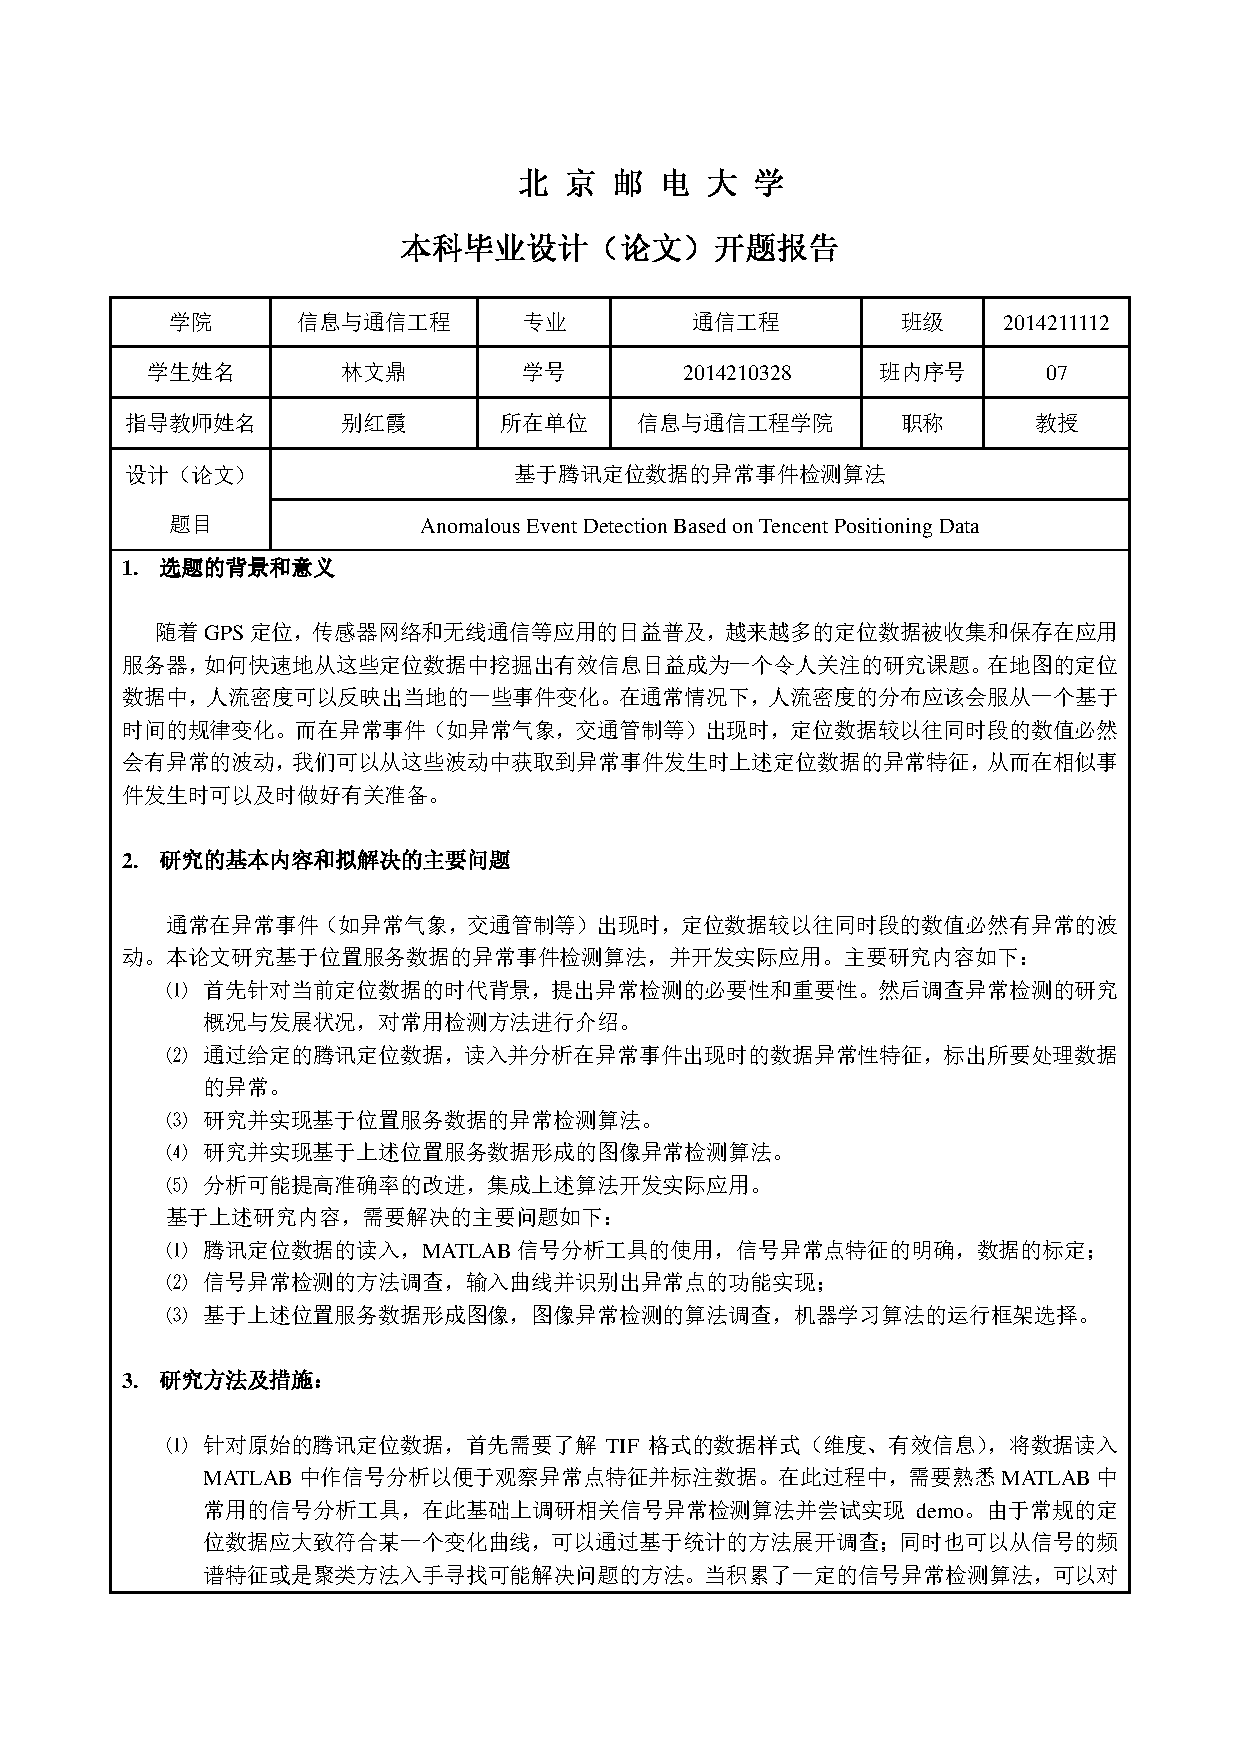
\includepdf[pages=-]{docs/openingReport.pdf} 


% 中期检查表
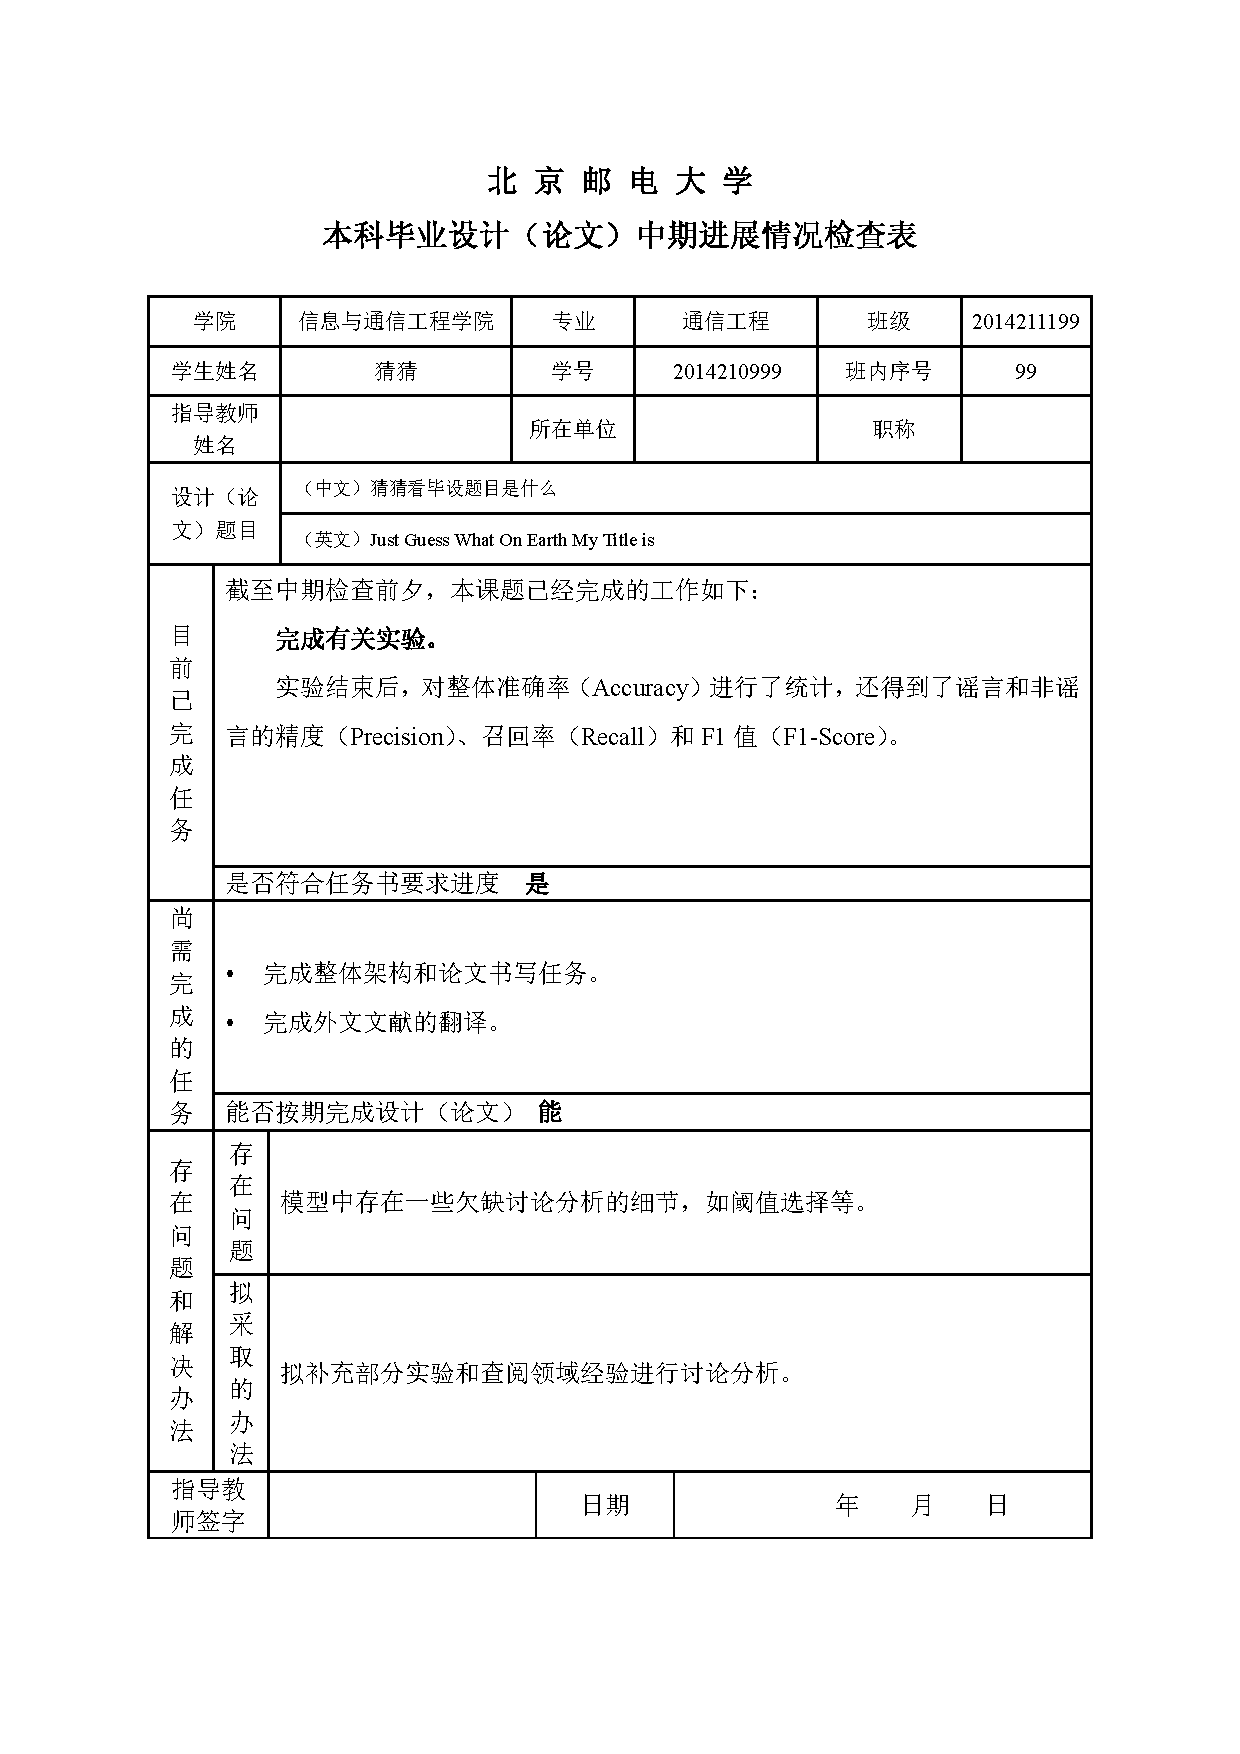
\includepdf[pages=-]{docs/interimReport.pdf} 


\end{document}
